\documentclass[12pt, a4paper]{report}

\usepackage{fyp}

%%these packages are not really necessary if you dont need the code and proofs environments
%%so if you like you can delete from here till the next comment
%%note that there are some examples below which obviously won't work once you remove this part
\usepackage{verbatim}
\usepackage{amsfonts}
\usepackage{amsmath}
\usepackage{amssymb}
\usepackage{amsthm}
\usepackage[hidelinks]{hyperref}
\usepackage{graphicx}
\usepackage{lmodern,textcomp}
\usepackage{algcompatible}
\usepackage{algorithm}
\usepackage{enumitem}
\usepackage{varwidth}
\usepackage{mathtools}
\usepackage[noend]{algpseudocode}

\usepackage{caption}
\usepackage{subcaption}




\makeatletter
\def\BState{\State\hskip-\ALG@thistlm}
\makeatother

\algdef{SE}[SUBALG]{Indent}{EndIndent}{}{\algorithmicend\ }%
\algtext*{Indent}
\algtext*{EndIndent}

\DeclarePairedDelimiter{\ceil}{\lceil}{\rceil}

%%this environment is useful if you have code snippets
\newenvironment{code}
{\footnotesize\verbatim}{\endverbatim\normalfont}




\graphicspath{ {images/} }

%%the following environments are useful to present proofs in your thesis
\theoremstyle{definition}
\newtheorem{definition}{Definition}[section]
\theoremstyle{definition}%plain}
\newtheorem{example}{Example}[section]
\theoremstyle{definition}%remark}
\newtheorem{proposition}{Proposition}[section]
\theoremstyle{definition}%remark}
\newtheorem{lemma}{Lemma}[section]
\theoremstyle{definition}%remark}
\newtheorem{corollary}{Corollary}[section]
\theoremstyle{definition}%remark}
\newtheorem{theorem}{Theorem}[section]
%%you can delete till here if you dont need the code and proofs environments

\setlength{\headheight}{15pt}
%\overfullrule=15pt

\begin{document}


%%make sure to enter this information
\title{Pin Pointing Pain Points: Vehicular traffic flow intensity detection and prediction through mobile data usage.}
\author{Maurice Saliba}
\date{28-06-2018}
\supervisor{Dr.~Charlie Abela}
\cosupervisor{Dr.~Colin Layfield}
\department{Faculty of ICT}
\universitycrestpath{crest}
\submitdate{28-06-2018} 

\frontmatter


\begin{acknowledgements}

I would like to thank my supervisor Dr.~Charlie Abela and Co-supervisor Dr.~Colin Layfield who taught me amongst many other things to let the data speak for itself. Discussing with them the various gradual achievements and caveats made it possible to foster insight.

I would like to thank GO p.l.c for supporting this dissertation by providing me with the anonymized mobile usage dataset and allowing me to use the high-end computing resources needed for the highly intensive processing required by this dissertation. I would also like to thank Dr.~Ing. Joseph C. Attard for encouraging me to pursue this Masters course. I also acknowledge the assistance of my colleagues at GO who were of great support and inspiration, especially when I discussed with them certain technical aspects of the project.

On a personal note, I would like to thank my wife Andrea for her great support, love and constant encouragement. I would like to thank also my parents, Benny and Carmen, and the rest of my family especially my nephew Kyle and niece Shirley who proved to be a useful forced distraction when needed. I would like to express my gratitude towards my close friends who did their best to drive me forward towards completion by constantly sending me pictures of them having beers on a great night out without me. 

Last but not least I would like to thank all the academic and non-academic staff of the department of artificial intelligence. It was a great academic journey that enriched my experience and perspective towards the world of science.



\end{acknowledgements}
       
\begin{abstract}

Multi-modal originated vehicular traffic flow data can be obtained with various techniques. To what extent this data is reliable, complete, timely and readily available hinges on thorough analysis of past work and currently available solutions. A novel approach, consisting of an ensemble of machine learning and data-mining techniques, is being proposed to prove that it is possible to extract vehicular traffic patterns from mobile usage data. 

An anonymized mobile phone usage dataset from a telecommunications provider in Malta is first used to carry out basic traffic analytics. Then an origin-destination (OD) matrix, based on the largest two clusters of activity per user, will be computed to infer user trips between these clusters over time. Routes for these trips are retrieved with open source routing tools, and obtained data pertaining to way nodes along these routes further enrich trip information. Spatial binning is then used to deduce the aggregate distribution of traffic load on the traffic network.  The OD matrix and grid network load are subsequently used to build a Neural Network predictive model. Several previous works \cite{Laurila2012,Hoteit2014} that carried out invaluable research in this field lacked on-line data in quality and quantity. They were at times compelled to devise corrective measures and carry out simulations to cater for such shortcomings. Having the luxury to avail of mobile call and data historical records made it more possible to fine tune a better predictive model and evaluate it. Industry standard visualization tools were used to portray AI generated traffic patterns together with flow intensity projected in the geospatial dimension.

The final results are satisfactory and the built models can effectively be used to both measure and predict traffic flow  counts in specific locations. Improvement through an addition of a dynamic traffic assignment algorithm to the proposed solution would give more accurate results especially for traffic flow points that tend to be congested. 
\end{abstract}

\tableofcontents

\listoffigures

\listoftables

\mainmatter



\chapter{Introduction} \label{chapter:introduction}

\section{Economic development and urbanization impact on transport} \label{section:introduction:economic_development}

Land transport is a societal reality that is essential for people to get to work, leisure and other places for other purposes. Transport is essential for delivering goods and services. Land transportation has undoubtedly evolved at a fast pace and late technology advancements are making vehicular transportation more efficient, less polluting, faster, safer and more comfortable. There are many land transport modes which include bus, rail and private car as the most generally used. In Malta 60\% of commuters opt for the car as the preferred mode of transport. This is stated in the modal split report in the National Transport Household Survey 2010 report document  \cite{malta2011national}.

Economic development and urbanization come at a cost. It surely has a direct impact on the increase of traffic congestion and all undesirable consequences it brings with it. Traffic congestion is especially synonymous with urban places where the private car is the preferred mode of travelling. The EU Transport Directorate (2018) mentions how traffic congestion in urban areas in the EU is costing 100 billion Euro every year which amounts to 1\% of the EU GDP \cite{EUTransportDirectorate2018}. Colak et al. elaborate on the crippling effect on the economy because of traffic congestion \cite{Colak2015}. Traffic congestion amounted to 43\% (\texteuro117.9 million) of external costs in Malta in 2012, which is the origin of the mobile traces datasource used in this study \cite{Attard2015}. Other causes of external costs related to traffic include accidents, climate change, air pollution and noise which are all directly incremented by traffic congestion. No policy change scenario envisages an external cost of \texteuro151.1 million and \texteuro154.1 million for the years 2020 and 2030 respectively incurred on the economy of Malta.

In the US, traffic congestion is similarly a cause of concern. Interesting but worrying facts are listed in a US mobility research done in 2015 \cite{Schrank.2015}. It states that the extra miles travelled by Americans in 2014 were 6.9 million at the cost of \textdollar160 billion. Congestion costs in the USA is on the increase. In the year 2000 it was reported to be at the level of \textdollar114 billion.

Traffic delays have a heavy impact on the shipment industry as well. Travel costs increase when travel time increases.  Pick-up and delivery time estimation become less accurate because of traffic congestion. Transport companies need to take costly measures in order to make up for this and the increase in cost is more often than not passed to the consumer  \cite{Schrank.2015, CambridgeSystematicsInc.2005}.

\section{Addressing Traffic congestion} \label{section:introduction:addressing_traffic_congestion}

Both car users and public transport users tend to get frustrated from unnecessary delays on the road. This time is deducted from a healthy lifestyle or from productivity hours. 

Drivers can adapt to smartly mitigate delay times. Individual drivers can hear radio adverts or check CCTV to inform themselves about the traffic situation before departing or while driving for better planning. Use of software such as Google Maps  \footnote{https://www.google.com/maps (accessed April 3, 2018)}, Apple Maps \footnote{https://apple.com/ios/maps (accessed April 3, 2018)} or Waze \footnote{https://waze.com/en-GB (accessed April 3, 2018)} help to have an informed decision how to schedule trips and decide what route to take.  These applications might even suggest other transport modes that offer faster or more convenient alternatives to get to the same destination.

Efficient traffic management should be at the top of national transportation agencies' agenda. Possible measures that can be taken by transport authorities include making different modes of transport more widely available and encourage the public to use it. Smart technology is another means to alleviate travelling frustration by giving information, instructions and control traffic flow in an automated manner. For more uptake of public transport the public for instance can be informed and educated through mobile applications.  Mobile applications can be used to make the public transport experience more efficient, practical and the preferred choice. There are other deterrents such as increases in vehicle license tax and adding of parking fees to force drivers off the road and make them use public transport or cleaner ways of transportation such as cycling.

Law enforcement is another way to facilitate traffic flow. This would diminish road accidents or casual road blockages that can cause flow disruptions. Automatic number plate recognition (ANPR), through camera feeds processing, can be used to measure traffic flow and even to apply a toll to users in certain traffic zones as a deterrent for private car use.  Park and ride systems shift away concentration of traffic from urban centres \cite{Attard2015}.  Nuaimi et al for instance show how concerted efforts can lead to smarter cities by analysing static data and make infrastructural changes by opening or modifying roads. In this study dynamic data was used to manage traffic lights to alleviate congestion, inform the public through their smart phones about the traffic status and control logistics related to movement of goods \cite{AlNuaimi2015}.

Investment in the transport infrastructure to expand capacity is difficult to directly justify with a simple cost benefit analysis model \cite{atkinson2006cost}. Increase in road capacity might seem a simple straightforward solution to alleviate traffic.  However infrastructure alterations might not necessarily equate to easing of traffic. Such costly changes might just spatially shift the problem elsewhere or fail to lead to the expected result. Forecasting of the gains made by road capacity increase or any other transport system changes may be distorted if induced traffic is not taken in consideration. Induced traffic may result from changes in route choice, peak hour traffic, modal split, overall transport volume, land use and quality of public transport services \cite{Naess2012}. When formulating return on investment functions induced traffic should not be ignored.


\section{Traffic information and management systems}\label{section:introduction:traffic_information_and_management_systems}

Traffic management systems primarily monitor traffic status in the road network and take traffic control decisions, such as, increasing or decreasing lanes in a tidal lane system based on traffic data. The traffic data, on which traffic management decision logic is based on, must be updated frequently and it should be reliable. Intelligent traffic management systems are more efficient when the traffic control decisions are based on real-time streams of traffic data. Processing real-time feeds is challenging both in terms of computational resources and design but is more reactive to abnormal situations such as accidents or unusual weather conditions since it is modelled on a running sample \cite{Toole2015}. Traffic related data stream processing might entail heavy real time processing of high variety data coming from multiple sources. Modern approaches, such as big data based information systems, become essential in order to create automated control systems that alleviate the load on the transport network\cite{Liu2014}.

Traffic Information Systems (TIS) can tap into mobile usage records as a main source of information. Such TIS leverage mobile data collection that has wide coverage, is reliable, accurate and is frequently updated  \cite{Leduc2008}. Less coverage is to be expected in rural areas where base stations are highly dispersed when compared to urban areas. Mobile vehicle geolocation has limited spatial resolution. For example it cannot be used for traffic flow counts on lanes, whereas it could be easily done with inductive loops. 

\section{Traveller centric traffic flow probing} \label{section:introduction:traveller_centric_traffic_flow_probing}

Obviously, the dynamics of traffic flow is determined by the travel needs of the masses. The daily commutes of every individual impacts those of others. The interaction on a large scale of all the vehicles in a time series is difficult to model and to predict in a robust and responsive manner \cite{VLAHOGIANNI20143}. Traffic sensors, cameras and induction loops are all sources of information that can be used to both detect high traffic intensity or even forecast it beforehand.  However, the coverage these techniques offer is limited. Camera feeds and inductive-loop detectors cannot be installed in every road of the transport infrastructure. Devices carried by travellers, or embedded in vehicle, can be possibly used to build smart solutions for traffic management \cite{VLAHOGIANNI20143}.


\subsection{Passive vs Active data collection}
Long before the information era started, spatio-temporal data on human mobility was collected in various forms and modalities. One of the methods used to gather such information is to do straightforward surveys\cite{Calabrese2013,Colak2015}. However these are expensive methods because a lot of manual work needs to be carried out. Besides they could only give a snapshot of reality at a given point in time.  Generally, these types of surveys are done every five to ten years \cite{Toole2015}. The data made available would be too static and increasing the frequency of survey taking would directly require more human resources assigned to the process. As mobile telecommunications and gradual adoption of its services came into the picture, at the turn of the millennium, more data points could be collected in an automated fashion. A limitation, which comes with mobile user related information, is the lack of demographic knowledge on the mobile owner. Surveys gather such information and make stratified sampling possible in order to have a more representative sample \cite{Colak2015}.

\subsection{Application of mobile traces analytics} \label{section:introduction:application_mobile_traces}

Mobile traces can be processed and used to offer location based services that have a wide application spectrum that go beyond solving mobility issues \cite{Hoteit2014,Calabrese2013,Gonzalez2008,Hoteit2016}. An individual's location and its relation with that of others within the context of the continuum of time is invaluable in many ways. This formidable datasource, however, poses a challenge. Location data, which usually comes in large amounts, has to be harvested, ingested efficiently and ideally processed in real time for the required final purpose which is value added location based services.

The range of application and branches of research abound on remote collection of mobile users' geolocation information.   To name a few applications include: traffic patterns and prediction modelling, crowd management, hotspot detection, lost device recovery, emergency rescue, use for investigative authorities,  location-based recommendation and advertising systems, contextualized information, social interaction based application, epidemiology etc.  

Calabrese et al  emphasized that studies on human mobility patterns would be vital for better sustainable urban planning and a boost for the environment's well being given that transportation in 2004 accounted for 22\% of primary energy use\cite{Calabrese2013}.

Steenbruggen et al mention how mobile geolocation data can be used to differentiate weekday traffic patterns from those in the weekend \cite{Steenbruggen2015}. Another specific type of  prediction based on mobile usage discussed in \cite{Hoteit2014} is jam detection.  Macroscopic monitoring and analysis of vehicle mobility through mobile traces is a wide area of study on its own which can branch in many fields of study \cite{Steenbruggen2015}.


\section{Problem definition}
From this research it is required to demonstrate that it is possible to attain an accurate measure of traffic flow and predict traffic flow for specific locations from predefined time intervals ahead. It is required to prove that this can be possibly done by constructing a predictive model and make use of inference techniques that base themselves on data usage records collected from the mobile cellular network. As we will expand in Chapter \ref{chapter:background}, the trajectory path plotted by the mobile antenna through which users are given service is far from being a true picture of the actual path of the user.  Another aspect of the problem is to detect when and where user trips start and finish and how this can be translated into traffic load on the road infrastructure.

An algorithm must be devised to deduce the actual path travelled by the user for his most common trips. The predictive model has to predict the traffic in a responsive manner since predictions that take a long time to compute will not be useful.


\subsection{Research Questions}

Research will be done in a direction outlined by the questions below:
\begin{enumerate}
	\item Is the resolution of mobile data usage cell tower location fit for purpose to measure vehicular traffic flow on the road network?
	
	\item How is it possible to extract the geolocation of main areas of activity from user's mobile data usage records?
	
	\item Is it possible to extract trip information that is based on the users' main areas of activity?
	
	\item What is the best approach to analyse traffic flow on the road infrastructure over time in space, given that trip information is available? 

	\item Is it possible to model traffic flow over time with machine learning techniques that use mobile data usage or processed data derived from it? How much time ahead can the model predict traffic flow with an acceptable margin of error in such a way that the prediction is useful and practical for trip planning and traffic management systems?
\end{enumerate}




\section{Aims and objectives} \label{section:introduction:aims_objectives}

In this dissertation we will focus on measuring traffic flow and predict how traffic flow changes over time for a selection of locations by using mobile data usage. A combination of data mining and machine learning techniques will be used to devise a data processing pipeline. This data processing pipeline will:

\begin{enumerate}
 \item consume raw event data records containing cell tower locations and date time and carry out preliminary descriptive statistical analysis. \label{objective:01}
 
 \item zoom into the main areas of activity of users by using unsupervised machine learning techniques that cluster the most dense groups of geolocation data points. \label{objective:02}
 
 \item  determine routes between these main activity areas and collect spatial grid aggregate data from daily trips done along these routes from thousands of users. \label{objective:03}
 
 \item use the transformed data which is representative of traffic flow in various locations to train and validate a predictive model using artificial neural networks \cite{Calabrese2013,Toole2015,Hoteit2014,Alexander2015}.  \label{objective:04}
 
 \item feed visualization tools that enable visual inspection of traffic patterns projected on maps. \label{objective:05}

\end{enumerate}

A selection of methods that are encountered in literature will be applied and evaluated. The real challenges arise in the quest for a high spatio-temporal resolution when modelling traffic, given that mobile usage records' geolocation dataset is sparse and tracks the position of users with a considerable margin of displacement error \cite{Hoteit2014,Gonzalez2008}.



\section{Dissertation outline} \label{section:introduction:dissertation_outline}
This dissertation started by introducing the reader to the problematic nature of vehicular traffic. It continues by expanding the socio-economic impact of traffic and how it can be addressed with modern technology. At the outset, it is mentioned how mobile data usage has great potential to monitor traffic conditions and to predict it over time.

 A background on traffic flow detection and prediction, and an overview of related literature, will be given in Chapter \ref{chapter:background} "Background and literature review". The proposed method to demonstrate the soundness of certain selected implementations of certain concepts inspired by literature will be elaborated in Chapter \ref{chapter:methodology} "Methodology".  Validity and versatility of the created model will be evaluated and discussed in the "Evaluation and Results" chapter.  The "Conclusion" chapter will summarize what has been achieved and to what extent in this dissertation, while highlighting limitations in the process. Finally, Chapter  \ref{chapter:future_work} "Future Works"  will discuss possible improvements and potential future projects that can build on the work done in this dissertation.



\chapter{Background and Literature Review} \label{chapter:background}

This chapter will go over mainstream techniques and approaches that make use of mobile data for traffic flow detection and prediction.

\section{Mobile location data sources} \label{background_mobile_location_data_sources} 

Network derived user location is an important attribute of a mobile cellular network. It is used to trigger call and data session handover and to enable a network to locate a user. Network paging is used to find the initial location of a mobile user. Other records are generated when there is a location update and hand over information \cite{Calabrese2011}. Network signalling records contains rich metadata to troubleshoot network issues. These records include also geolocation data. 

From a telecommunications background perspective there are two types of generated records.  These types are call data records (CDR) and event data records (EDR). An EDR, differently from a CDR, comprises other forms of activity other then calling. Both CDR and EDR data are generated by network elements to capture and report user activity within the network. Reporting frequency and record triggering events can be configurable, allowing operators to trade off between keeping at their lowest the quantity of generated records that are hungry of storage resources and providing enough data for billing/troubleshooting purposes.

Mobile internet is the service that generates most records. As soon as the user connects to the network, a first record is generated, providing all of the available information, including which cell tower is providing the service. Since data sessions span over a long period of time, periodic updates are required, allowing billing related entities to control whether the user may continue to make use of the service or not. These updates may be triggered by either of the following:
\begin{enumerate}
\item Volume - a new record is generated as the user consumes more than a pre-configured volume.
\item Time - if the user is idle, a new update record is still generated after a specific amount of time from the previous record.
\item Network Trigger - operators may decide to generate a record each time there is a specific change (for instance, a change in radio access technology)
\end{enumerate}
	
Together with call records, SMS records (messaging) and data traffic (2G/GSM, 3G/UMTS, 4G/LTE) records can also be stored. SMS records structure are similar to those of CDRs \cite{Calabrese2013}. A CDR structure would include the A-party (who is calling), the B-party (the person who is receiving the call), call duration, date and time of calls amongst other things which might not prove to be useful for location deducing purposes. The location is implicitly the sector of the base station antenna which was managing the call/sms and where ultimately the CDR has its origin. The trigger for a cell handover or for a 4G to 3g or 2G handover is dependent on the received signal strength as well as cell congestion \cite{Liu2014}. This has an implication on location detection as we will see later on. A data event record would include volume of transmitted data in the session.

Mobile device location traces have their limitations when used for vehicular traffic analyses. In contrast to surveys, they lack demographics \cite{Calabrese2013,Colak2015} and market share of the mobile service provider that made the dataset available for scientific research might not be really representative of the commuting patterns \cite{Calabrese2011}. Many studies highlighted the importance of removing bias when preprocessing such datasets before any further processing is done \cite{Iqbal2014,Toole2015}.  Passive data, gathered in the form of CDRs, are not suited to extract different modes of travel, route assignment and classify detailed activity types \cite{Colak2015}.

Mobile device location data is not only limited to data that originates from cellular networks. Global positioning system (GPS) is the most reliable source of geolocation because of its higher resolution with lower margin of error. This data is generated by the device and needs to be stored and communicated from the user's mobile with his own specific authorization. Using GPS data for a mobility study is more challenging because it needs the consent of users to get such data and drains the battery quickly especially because of long signal acquisition time\cite{Wang2012}. Thus users would be reluctant to have such service running in the background on their mobile phones all the time \cite{Ahas2011}. 

CDR data was the mobile location data source mostly used in recent research \cite{Hoteit2016}. The intention of our research is to use data usage EDRs since these can have a higher temporal resolution. CDR data can be more commonly generated when a user is not moving unless he is using hands free in his car. CDRs therefore would be more suited for home and work location detection whilst data usage records would be more generated frequently both when user is moving and stationary. From the literature review it results that most research projects use voice CDRs to trace mobility. Research projects that were found to rely on mobile data usage to detect vehicular traffic or predict it include \cite{Hoteit2014,Calabrese2011}.

Other sources of geolocation include social mobile application recorded events such as check-ins in facebook \cite{Hoteit2014}. Such data can be accessed by available APIs \footnote{https://developers.facebook.com/docs/graph-api/reference/v3.0/checkin (accessed April 7, 2018)}.

\subsection{Mobile usage data format and dataset sample structure} \label{methodoloy_sources}


It is important to analyse in depth the structure of mobile records dataset sample and the method of collection thereof in order to understand possible limitations and strengths in related research. Another topic of special interest is the use of secondary datasets used to validate results achieved when modelling travel on mobile generated data. Hoteit et al utilized mobile data coming from 1 million users between July and October 2009 \cite{Hoteit2014}. The data consisted of calling and messaging parties' anonymous id together with data of when users made a data session. Calabrese et al. (2013) used data originating from CDRs (a sample of 1 million mobile users in Massachusetts) which included calling id, time of when call/sms was sent or received and when a data session is initiated. Interestingly Calabrese et al. (2013) used vehicle safety inspection data as well. This data was used especially for evaluation. Vehicle safety inspection data was later used to approximately verify the kilometres covered by inferring the trajectory. The time window used by \cite{Calabrese2013} was 3 months long and the  area under study was metropolitan Boston.

Calabrese et al and Colak et al stressed several reasons why research data samples collected with surveys present a lot of disadvantages when compared to mobile device generated data including sample size which is smaller, update frequency and certain types of time windows that are seldom considered or not captured by surveys such as seasonality, public holidays and weekends \cite{Calabrese2013,Colak2015}.   

Gonzalez et al mention two datasets in their research. The first sample was of 100,000 individuals sub-sampled from a wider dataset population of 6 million anonymized  phone users. Similar to other research aforementioned, the data which was used included id of device from which calls or sms originated or terminated and location of tower projected over time. The reported average area covered by a cell tower was 3 km$^{2}$ with 30\% of cell towers having a coverage of 1 km$^{2}$ or less. The second dataset consisted of 206 mobile users whose actual location was traced every two hours for a week. By comparing analysis of this dataset to the first one Gonzalez et al found irregularity in calling patterns observed when using CDR data only. Displacements were recorded for consecutive calls in order to construct a travelled distance distribution model.

Hoteit et al use two datasets which have GPS location of 86 mobile users in various places in the world \cite{Hoteit2016}. One dataset is generated by sub-sampling the original one in order to emulate a sparse CDR dataset. Authors were forced to do this since no real CDR dataset was available for their research.  

In literature two different types of tools have been found to be employed to aggregate location data. Airsage datasets were found often to be used in literature \cite{Hoteit2014, Wang2013, Calabrese2013,Leduc2008,Wang2012, Colak2015}. Basically Airsage does not simply just record the tower cell sector but depending on a refined triangulation algorithm it gives a more precise location.  \cite{Hoteit2016} makes use of MACACOApp which is an app that records mobile data usage but most importantly also GPS data. As already aforementioned GPS technology gives a more accurate geolocation. However the data sample size is smaller in comparison to data samples collected in the form of raw CDR data in other studies.

\subsection{Mobile position inference from Floating cellular data} \label{mobile_inference} 

Collection of localization data that makes use of mobile phone data connectivity with base stations is commonly referred to as floating car data or more specifically floating cellular data (FCD) for sensor data originating mainly from cellular networks. A specific technique to actually determine a user's location is based on triangulation as done by the Airsage solution \cite{Hoteit2014}. An intuition about triangulation is shown in Figure \ref{fig:triangulation} which is reproduced from an article by Phil Locke\footnote{http://wrongfulconvictionsblog.org/2012/06/01/cell\-tower\-triangulation\\-how\-it\-works (accessed January 14, 2018). The red ellipse is the location boundaries for the phone}. Proprietary algorithms process data received from mobile service providers and outputs refined location information to customers. It was reported that in testing carried out by Geostat Inc. Airsage got accurate classification of congested traffic 91\% of the time  \cite{Wang2012}. No technical background was made available on how these algorithms get a more precise location of mobile users and this is most likely attributed to the fact that the algorithms behind the solution are patented \footnote{https://patents.justia.com/assignee/airsage\-inc}.  

\begin{figure}[!] 
	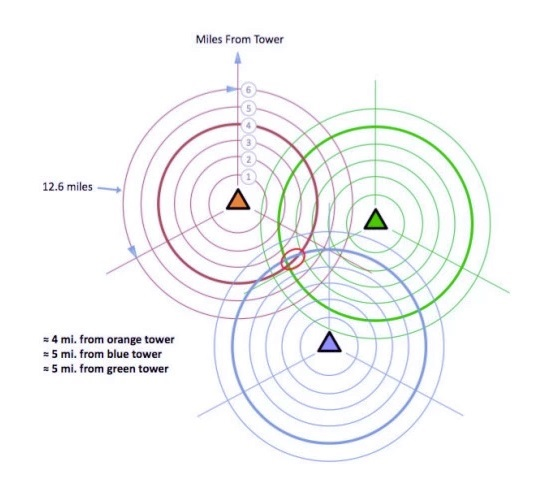
\includegraphics[scale=0.75]{triangulation.jpg}
	\centering
	\caption[Triangulation concept]{
		Illustration of the triangulation concept which is based on signalling and negotiation with nearby towers. Triangulation computes the location information inferred from signal strength experienced by the mobile phone user. If no second or third tower was present the location would be considered anywhere within the sector on the circumference that is demarcated by the signal strength. The red ellipse is the location boundaries for the phone.}
	\label{fig:triangulation}
\end{figure}

It is stated in \cite{Colak2015} that Airsage location computation accuracy is within 200 to 300 metres . Calabrese et al state that the degree of location precision reported by AirSage is an average of 320m and median of 220m \cite{Calabrese2013}. As already aforementioned, AirSage has been used in \cite{Hoteit2014} as well. In comparison \cite{Gonzalez2008} simplistically mentions that 30\% (average is \(3km^{2}\)) of the towers are placed in a density of 1 tower per square km. This roughly would mean that, at most, an unprocessed location retrieved from cellular location data would have a maximum error of around 500m. 

Location given by cell tower position, to which mobile phone user is connected to, is not useful for precise localization since recorded geolocation might be hundreds of metres away from the actual position. In our research we cannot make use of Airsage datasets. Such solutions must be already in accordance with mobile network operators from where mobile usage data is acquired.

Therefore, in this research some effort had to be dedicated to devise a simple triangulation or clustering method that can achieve more accurate mobile user location than the actual cell tower location. Since the grouping of multiple mobile users within a grid of location cells is more practical in giving a more clear traffic flow measure an essential topic to treat in traffic congestion research is spatial binning. Spatial binning determine geographical aggregate statistics. 

MapReduce frameworks such as Spatial Hadoop exist so the expensive temporal geospatial analytics are done within an acceptable time window \cite{Wu2014,eldawy2015spatialhadoop}. Such tools provide the possibility of doing spatial joins that can correlate spatial features extracted from sources such as OpenStreetMaps with mobility data from a mobile usage dataset \cite{Alarabi2014}.


\section{Privacy and data anonymization} \label{data_anonymization} 


Mobile subscribers location and CDRs are highly sensitive data, therefore anonymization is required to protect the privacy of individuals when using such data for research purposes. Some standard practices that make anonymization procedures more robust are listed in Laurila et al \cite{Laurila2012}. For instance Laurila et al exposes facts regarding potential privacy breach risks within datasets that have unique identifiers hashed.  One of these is contractual binding where data users are legally bound to not attempt to reverse-engineer identity. Another method to further protect sensitive data through anonymization is truncation of data. For example only a part of the data is kept if it is decided that it is enough and meets the purpose of the data processing exercise. Also Laurila et al also give a detailed account of techniques used to hash unique identifiers. Shin et al. elaborates on how to use k-anonymity algorithm so that location data of a user makes his identity undistinguishable from other k-1 other users in the same region \cite{Shin}.

Another way to guarantee privacy is limiting data retention. To safeguard privacy travel paths of a specific mobile user is kept for not more than 1 day in \cite{Hoteit2014} and for not more than 2 days in \cite{Calabrese2013}. It is the norm to assign a hashed anonymous identifier to each mobile user in such a method as well.


\section{Big Data, the cloud and large scale real time stream processing} \label{background_big_data}

Liu Jun et al expand on the recent phenomenon of computing systems not keeping up the pace with the vast increase in storage requirements \cite{Liu2014}. In this study it is explained how intensive computing speeds are compromised when there is a lot of data reading and writing and when it is required to move both input and output data around in a distributed system for further processing and consumption. 

Big data frameworks are suited for such scenarios. It shards the volume of data on a cluster of nodes and makes the addition of a new node in the infrastructure seamless. Failure of a node will not disrupt an ongoing global process since data will be redundant. Data redundancy is implemented by replication of data in blocks residing in nodes across the cluster. Hot replacement of failing nodes is also a smooth operation in big data infrastructure. The main paradigm shift to attain a high performance gain was to limit distribution of data across the network because this would mean less efficiency because of network transmission latency. The main strength of new Big Data architecture resides in offloading processing to the nodes where the data is located and only the resulting required information is transmitted back to a centralized node where the driver program is \cite{inoubli2016experimental}.

When is the data infrastructure of a system in need of a shift to the Big Data paradigm and traditional RDBMS systems cease to be the preferred choice? When you have the 3 V's which are volume, velocity and variety in the data is a recipe for big data introduction as a part of the solution. This is quite applicable to the processing of the multitude of mobility data which comes in huge amounts and need to squeeze out information in the least amount of time. Our dataset that was collected between August 2016 and September 2017 is 150 GB in size. Building a predictive model on this dataset of such size and retrain in real-time would require a big data solution. 

Currently some of the leading frameworks in this area are Hadoop and Spark. Hadoop is treated in detail in \cite{Liu2014} and revolves around the MapReduce programming model. This work shows how enormous amounts of data is stored in a distributed fashion on HDFS (hadoop file system) which is highly scalable and fault tolerant. Spark is used extensively in lambda architectures that include both nightly batch and real time batch processing. Liu Jun et al research is not directly related to the analysis of mobility behaviour but describes well how to process mobile device generated data traffic \cite{Liu2014}. It also gives a good account on how to monitor the infrastructure through various metrics and tooling. There are many papers related to mobile user travel pattern prediction that make use of big data innovation  \cite{Liu2014,Laurila2012,Kurien2012}. Toole et al. \cite{Toole2015} state that dataset size can be an issue for computation when determining the origins and destinations (OD) matrix (refer to Sections \ref{section:odmatrix_trip_generation} and \ref{section:OD_Matrices}). In this same study parallelization is used to assign routes to trips.


\section{Origin and destination matrices computation} \label{section:OD_Matrices}
A consistent recurrence in traffic flow analyses literature is the study of how to deduce origin and destination (OD) locations for travelling vehicles \cite{Iqbal2014}. Many research articles confronted the problem posed by traffic congestion detection by first deducing the OD matrix \cite{Toole2015,Iqbal2014,Alexander2015,Calabrese2011,Calabrese2013,Colak2015}. 

\subsection{Use of OD matrices to store information on main user locations and trips inbetween}

ODs are used to extract main activity hubs. Gonzalez et al state that 40\% of the time users are at their two preferred locations \cite{Gonzalez2008}.  Therefore most trips can be mostly explained as being  between several locations since users tend to be highly inclined to be regular in spatial and temporal terms. All this leads to safely assume that the majority of trips are between home and work. In literature it  is commonly found that locations that were likely to be recorded in OD matrices were home and work \cite{Calabrese2011,Colak2015}.  In \cite{Calabrese2011} home location is detected for user by checking which 500 metres square cell has the most activity during the night for every specific user.

Colak et al label zones such as home and work and tries to find purpose behind other types of trips \cite{Colak2015}. In this work it is mentioned as well how ODs are analysed in terms of stays and trips. Frequency of calls and time of day determine the labelling of these stays. It is stated that it was not possible to categorize other types of stays other than home and work. So these types of stays were labelled under the 'other' class.

Calabrese et al (2011) put forward the concept of virtual location which is derived from fused visited locations by the user \cite{Calabrese2011}. This research devises an algorithm that localizes the centroid of important locations in a user trip that are to be labelled as the origin or destinations of particular users. The method analyses which points are in the proximity of others within a 1 km radius. 

 


\subsection{Cleaning of data, removal of noise and minimization of displacement error} \label{subsection: data_processing}
A common occurrence in literature is to remove users that do not make enough mobile usage. The behaviour of these is less predictable and its more difficult to generate trips from OD data for this type of users. In \cite{Toole2015} users that do not make enough calls are filtered out from the dataset and \cite{Colak2015} filters out users with low activity when labelling activity zones.

Displacement errors due to sudden change of cell tower for various reasons are reported to make datasets inconsistent. False displacements are reduced in \cite{Iqbal2014} by using a time window of 10 minutes. The most common location in the 10 minute window was considered the actual location. A time window of 1 hour is than used to detect trips. In \cite{Calabrese2011} a low pass filter is used to minimize localization errors. To reduce sudden movements due to cell tower handover clustering is used. The same concern is raised in \cite{Colak2015} in a similar fashion and decribe how CDR data contains jumps or oscillations which introduce noise in the dataset. 

It is mentioned in \cite{Colak2015} how Airsage dataset inherently provides triangulation that gives medoids as processed data. Filtering out of noise in a Rio de Janeiro CDR dataset is done by labelling stays only if records are registered for a user for more than 10 minutes. When observing stays for users for a longer period of time it is possible to get more clear patterns where the stays are actually visited by users or not. \cite{Toole2015} removes noise from mobile phone calls deduced trajectories by using the stay algorithm proposed in \cite{Zheng2011}. A location is labelled as a 'stay' whenever user makes a set of calls within a time window greater than a given threshold. The centroid is then calculated for a set of locations that are close to each other in order to compute a better approximate location of the user. In \cite{Iqbal2014}  estimation of OD matrices can be found to be unreliable because of sampling bias. Equally \cite{Toole2015} stresses that bias needs to be removed when constructing OD matrices.

An important attribute to consider in OD matrices is its resolution since it might be important to aggregate data for statistical purposes. Not a lot of information was found in literature on this. In \cite{Colak2015} census tracts and town boundaries are chosen for OD resolution level. No justification for this choice is given tough.

\subsection{Use of scaling methods to get more accurate OD matrices} \label{subsection:OD_scaling}

%TODO - why are you scaling? Not clear enough.
Scaling methods to scale traffic flow counts are often used to obtain OD matrices that reflect reality better. In \cite{Iqbal2014} a scaling factor $\beta$ was used to get an OD matrix for the scaled up traffic flow between nodes. Traffic flowing from node $i$ to node $j$ was scaled up by this scaling factor $\beta$. The scaling factor is obtained by inputting optimization formulas, route choice probabilistic models, network data and the original OD matrix in a simulation engine. The scaling is then distributed as shown in Equation \ref{OD_scaling}

\begin{equation}\label{OD_scaling}
\textit{OD}_{ij} = \sum _{ij} (t-OD_{ij}) * \beta_{ij} 
\end{equation}

In Equation \ref{OD_scaling}, $OD_{ij}$ is the final resulting actual OD matrix.  $(t-OD_{ij})$ is the transient OD matrix that contains trip data from origin nodes to destination nodes. Transient here means that the node to node trips may be missing the actual nodes' information because CDR data does not capture all locations in the trips made. Thus $(t-OD_{ij})$ represents only a segment of the actual trips. $i,j$ represent different links between nodes. A simulation platform, MITSIMLab\footnote{https://its.mit.edu/software/mitsimlab (accessed November 14, 2017)}, was used to find a scaling factor $\beta_{ij}$ for every transient OD link.

Colak et al uses the iterative proportional fitting (IPF) upscaling method \cite{Colak2015}. Here Colak determined the expansion factor for each tract and in the IPF took in consideration trips to destinations as well. In his conclusions Colak stated that the IPF Procedure to distribute user CDRs according to population might have been too simplistic of an approach.


\subsection{Route selection for OD matrices}
Route selection is necessary to link origins and destinations from OD matrices to generate OD trips. In \cite{Iqbal2014} route is determined by a function of least travel time path. In \cite{Toole2015} Open Street Maps\footnote{https://www.openstreetmap.org (accessed December 7, 2017)} (OSM), which is an open source map editing framework, is used to infer routing. Some studies assign trips to a user when there are consecutive calls in the same day and the calls are done from different locations. An example approach is that two consecutive 'stays' that are not more than 1 day apart would constitute a trip \cite{Colak2015,Toole2015}. 
OD matrices determined trips would not be sufficient to model traffic on a network. Microscopic traffic assignment dependent on these trip generation exercises needs to be modelled. Toole et al for instance implements incremental traffic assignment (ITA) in which trips are added to network incrementally \cite{Toole2015}. Then on each iteration routes are assigned according to capacity saturation of roads. It is admitted however that Wardrop's equilibrium  adapts better since routes are changed dynamically depending on congestion. However ITA algorithm is chosen because it is simpler to implement. Colak et al relies on a probabilistic model for traffic assignment. Departure times for trips are set according to pre-set distribution of departures \cite{Colak2015}.


\subsection{OD matrices evaluation}

Evaluation related to OD matrix generation is generally done by correlating the generated locations and trips to survey data. In \cite{Toole2015} survey data traffic load on road network is compared with that generated through OD matrices formed from mobile CDRs. Simulation generated routes for the latter have been produced with the ITA approach. In \cite{Toole2015} it is stated however that other methods should be further explored to removed uncertainty from the proposed techniques.

In \cite{Iqbal2014} traffic count was collected on a spread of 3 days in 13 locations and this data was used for calibration of the system.  For validation another day was used with 4 different locations. Prediction root mean square error (RMSE) and root mean square (RMS) percent errors were 335.09 and 13.59\% respectively. In \cite{Calabrese2011} evaluation was done against a tract by tract census. Euclidean distance was calculated and the distribution of the trip distance confirms Gonzalez affirmation that trips follow a random walk \cite{Gonzalez2008} which is discussed in section \ref{section:human_mobility_modelling}  (See equation \ref{equation:random_walk}).

\begin{equation}\label{equation:random_walk}
P(x) = (x+14.6)-0.78^{-x/60}~ with~ R2 = 0.98 
\end{equation}

Here euclidean distance added error and to have it visualized with lines emanating from and linking nodes, although it might prove to be simpler, it would not give more insight on the road infrastructure use. In the OD trip analysis done by \cite{Calabrese2011} it is estimated amongst other things that a user makes 5 trips on weekdays and 4.5 during the weekend. This matches approximately the US census data which is 4.18 during weekdays and 3.86 on weekends. Study concludes that the OD matrices that are produced with the proposed methods can be of great value to those who are responsible for traffic planning.

Colak et al carried out evaluation against traffic surveys and already available OD matrices from department of transportation \cite{Colak2015}.  The validation however was done against a morning sample. Colak et al boasted of trip generation and attraction correlation near to 1 for both cities in study namely Boston and Rio de Janeiro. The correlation with already validated datasets is highest when OD matrices are generated from aggregations done on larger polygons. 

Colak et al reported OD matrix limitations. Suitability of CDRs to determine ODs is only good at a certain resolution. It is stated that better results are attained when using higher resolution for home or work location detection and aggregation within larger zones (towns or districts) for OD trips representation. OD matrices are less fitted to get information on the whole travel model which for example includes modal split information.


\section{Traffic flow measurement and pattern extraction}
Traffic flow measurement can be explained in terms of vehicle count per \textit{t} amount of time or even in a more descriptive way with a metric that measures travel performance as volume over road capacity V/C \cite{Toole2015}. The latter metric has more information since a road with low capacity may be more congested than another that has the same rate of traffic flow but a higher capacity. In a more elaborate metric proposed by \cite{Toole2015} a road can be possibly classified as a function of betweenness and usage. Classes are defined as connector (high betweenness and high usage), attractor (low betweenness and high usage), peripheral (high betweenness and low usage) and local (low betweenness and low usage).


\section{Model fitting to human mobility} \label{section:human_mobility_modelling}
Mathematical modelling of human mobility is important to predict with a stated certainty the location of a mobile user in time since data collected from mobile devices is sparse. Interpolation methods were used to describe human mobility patterns in \cite{Hoteit2014}. These are namely linear-interpolation, nearest-neighbour interpolation and cubic interpolation. Linear-interpolation would simply project the mobile user position at time (t) by plotting a straight line from the last previously recorded location and the one right immediately after. This method's error margin is widened if data collection time interval is longer for data points pertaining to the same individual that is moving. As for the nearest-neighbour method, location is attributed to the previous recorded value or to the subsequent depending which is the closest on the time axis. The cubic interpolation is best explained when contrasted with the linear one. This method as explained in \cite{Hoteit2014}  is described as "shape preserving". The slopes shaping the curves are deduced from derivatives and give a less sharp demarcation and better guess depending on a series of data samples.

In \cite{Gonzalez2008} both the variation of displacements for consecutive 'steps' (i.e. call location and respective time at which call is made) and the radius of gyration distribution was modelled as truncated power-law which is referred to in all the work as a levy-flight (See Figure. \ref{fig:levy_flight} and Equation \ref{displacement_distribution} for illustration of displacement distribution modelling). A levy-flight is a random walk where the probability distribution of the steps taken is heavy-tailed. This model explains what is the probability distribution $P(\Delta r)$  of the distance travelled from radius of gyration by individuals who travel as far as 400km ($D_1$) and those who travel as far as 80km ($D_2$). $D_1$ and $D_2$ are cutoff values. 

\begin{equation}\label{displacement_distribution}
P(\Delta r) = (\Delta r + \Delta r_{0})^{-\beta}  exp(-\Delta r/\kappa)
\end{equation} 

with exponent $-\beta$=1.75 $\pm$ 0.15 (mean $\pm$ standard deviation), $\Delta r_{0}$=1.5 km and cutoff values $\kappa|_{D_{1}}=400 km$ and $\kappa|_{D_{2}}=80 km$ 

\begin{figure}[h]	
	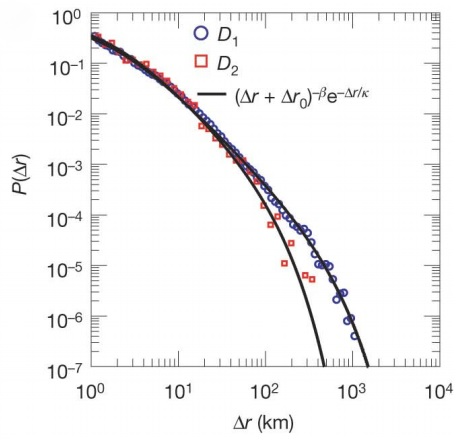
\includegraphics[scale=0.75]{truncated_power_law}
	\centering
	\caption[Truncated Levy Flight]{Truncated levy flight human motion modelling. Reproduced from \cite{Gonzalez2008}}
	\label{fig:levy_flight}
\end{figure}


This mathematical model is cited and verified in \cite{Calabrese2013}. The methodology adopted in \cite{Hoteit2016} suggested approaches how to determine home and work locations, span of movement and complete trajectory. Two datasets were compiled. One dataset is a sub-sample of another dataset which has a higher resolution because it has been composed of GPS geolocation data. The sparsity of the second dataset have been mimicked by a cumulative distribution function in order to create a virtual CDR dataset. Only users with high activity were considered in order to have less irregularity. Home and work locations were determined with a mode function with catch-all time boundaries for day and night where supposedly users are either at work or home respectively. For span of movement a similar mathematical approach was adopted as the ones in \cite{Hoteit2014,Gonzalez2008}. As for the actual movement trajectory error was calculated by calculating the euclidean distance of each CDR data-point from the actual GPS recording which is nearest in time.
Some techniques were used to lessen the margin of error. Since most of the time the typical mobile phone user is static, data completion is attained by applying a list of inference rules for which different results are achieved when estimating users location, hence the name of the paper "filling the gaps".

A problem was outlined in \cite{Calabrese2013} about detecting a lot of trips in very short distance which do not reflect statistical data given by surveys. This is explained as being caused by fluctuating random connections with towers which spatially misplace the user when in reality he is not actually physically moving. This issue was tackled by mathematically creating so called by \cite{Calabrese2013} 'virtual locations' (a mass/group of traced positions in a given radius of Airsage resolution) and actually recording a movement when user moves from a virtual location to the other. Calabrese et al limit static location detection to the home location and the proposed process how to manage to get each user's location is similar to that expounded in \cite{Hoteit2016}. In a novel style this work studies the relationship between total trip length calculated from mobile phone location data and vehicle kilometres travelled (VKT) and urban features such as entropic type, population density, intersection density, average distance to non-work destinations, distance to subway stations and highway exits. These urban features were derived from US Census of 2000 and activity travel surveys.

Estimation of load error is proportional to concentration of users in a given block \cite{Hoteit2014}. For recorded error with value less than 1 km a probability of 80.78\% of being within commonly travelled territory contrasts with a probability of 19.22\% when user travels outside of it. From the opposite perspective of having error greater than 1 km, the probability of being inside radius of gyration was found to be 40.25\% and that of being outside is 59.75\%.

In \cite{Calabrese2013} results state that 49.40\% of mobility variation can be explained for individual mobile users and 56.48\% for vehicle associated mobility in terms of trip length.    

In \cite{Gonzalez2008} results point to the phenomenon that the greater is the radius of gyration the less symmetric in shape is the probability density function which gives the probability of a user being in a given location (x,y). Also the margin of error increases similarly as stated in \cite{Hoteit2014}. It is also shown how individual mobility is well described by a levy-flight. Also a probability density function has been implemented to give the likelihood a user is at a certain given place in time.

The techniques used to further refine the location based on the assumed location home interval gives results in the range of 92\%-95\% of cases within 100m \cite{Hoteit2016}. Techniques will produce large errors (in the range of 50km) when user travels long distances and may not return to home location during the usual time interval.

Error distance from trajectory depends on radius of gyration \cite{Hoteit2014}. Interpolation methods are found to be most suited depending on distance from the geometrical centre of all the movement. Nearest neighbour is most suited for $r_{g}$ less than 3 km. Between 3 km and 10 km both linear and cubic interpolations perform well. For commuting travelling patterns trajectory is best estimated with a cubic interpolation.
Interesting insights were contributed in \cite{Calabrese2013} where it is stated that job accessibility and distance to non-work destinations are inversely proportional to total trip length. Distance from subway does increase trip length for individual mobile users but it does not impact vehicle use. This means that subway commodity does not necessarily decrease vehicle use in the surrounding area. Vehicular trip length decreases when correlated with increase in intersection density but not so for individual mobile users. Urban entropy and population does significantly impact trip length. Thus this study can help a lot in urban planning and large scale policy making.
In \cite{Hoteit2016} it is affirmed that the solution of data completion augmented by the placing of users in their home location at inferred intervals of time produces better results then what was achieved in literature.

There are many approaches in literature how to classify group mobility patterns under specific categories. Hoteit et al (2014) segmented mobile users depending on the width of the radius of gyration (\(r_{g}\)). The different distinguished categories of users are listed as sedentary, urban, peri-urban users and commuters. The classification boundary was decided upon steep changes in the cumulative distributed function of the radius of gyration. Respectively these classification labels fall in the ranges \(r_{g} <= 3km, 3km < r_{g} <= 10km, 10km < r_{g} <= 32km, 32km < r_{g}\) \cite{Hoteit2014}. The radius of gyration (see eq. \ref{radius_gyration}) is the notion outlined by the sum of all displacements from the centre of mass divided by the number of trips. This parameter describes how distributed are the trips far away from the zone where the user mostly frequently returns. Repeated utilization of this mathematical notion is found in \cite{Hoteit2014,Gonzalez2008,Hoteit2016}.

\begin{equation} \label{radius_gyration}
r_{g} = \sqrt{\frac{1}{n}\sum _{i=1}^{n}({\stackrel{\to }{p}}_{i}-{\stackrel{\to }{p}}_{centroid})^2}
\end{equation}

where 

\begin{equation}
{\stackrel{\to }{p}}_{centroid} = \frac{1}{n}\sum _{i=1}^{n}{\stackrel{\to }{p}}_{i}
\end{equation}

where $r_{g}$ is the radius of gyration and ${\stackrel{\to }{p}}$ is the magnitude of the displacement vector.   

In \cite{Hoteit2016}, the hypothesis that an individual tends to be found with high probability at his home or place of work leads to classification of individual calling activity locations. The classification method labels these locations as \textit{'stop-by'} categories. The 'stop-by' category 'stop-by home' is demarcated by the night time interval where a user is expected to be at home. 'stob-by-flexhome' is a refinement over and above 'stop-by-home' were night time interval varies per user. 'Stop-by-spothome' fills data gaps or corrects errors when there are exceptional errors where user is expected to be in home location, as indicated by previous category.



\chapter{Methodology} \label{chapter:methodology}

One of the main objectives (O\ref{objective:01}) was to extract meaningful features from mobile data usage that would serve as the basis to build a traffic flow model. Before choosing an approach and constructing an algorithm that maps raw data and translates it into traffic flow metrics a thorough familiarization exercise with the data was due. A feasibility check had to be carried out on whether it was possible that by devising an algorithm a direct relationship is established between mobile usage data and traffic flow. If data was found to be too sparse, both temporally and spatially,  augmentation would have been required by tapping into other datasets would have been necessary. Such  datasets could include ANPR data collected from video streams, call data records available openly on the internet, accident reports and anything related to road transport which would convey additional information on human mobility patterns. 

In this chapter we will elaborate how we investigated a number of approaches and how we decided to dig deeper with a set of techniques preferred to others depending on how practical the solution was and how it would give a better result. The methodology presented in this chapter has a step by step scientific method in which procedures were devised to test hypotheses. The data that results from a devised procedure was analysed and if it was not working properly further optimizations were done and alterations were discussed. Finally conclusions were drawn and communicated in Sections \ref{chapter:evaluation_and_results} and \ref{chapter:conclusion}  and where results were not found aligned or partially aligned with the hypotheses, suggestions how further research can be done were outlined in Section \ref{section:future_improvements}. 

The main hypotheses' experimental procedures that have been tested and refined in this methodology are 

\begin{enumerate}
	
	\item Clustering of main user activity locations. 
	\item Trip generation from main activity clusters.
	\item Trip count and trip delay measurement.
	\item Traffic flow load distribution on road infrastructure. 
	\item Traffic flow prediciton with different prediction time interval ahead.
	
\end{enumerate}

\section{Mobile data collection and structure} \label{section:methodology:mobile_data_collection_structure}

The anonymized dataset was provided by GO Plc Malta\footnote{https://go.com.mt (accessed May 4, 2018)} which is one of the main Maltese telecommunication services providers. The anonymization process was done by the company itself and authors had no access to the original dataset. The dataset recorded ranges from October 2016 to September 2017 which is a full year of data. However it was decided to concentrate only on the month of October 2016 so that analysis and model learning is faster by working on prototypes tested on a sample of the data. The data volume for the month of October was 11 GB. The whole dataset volume amounted to 150 GB. Notwithstanding the fact that all experimentation was only done with data from October 2016, results were considered to be satisfactory even though it is known that for certain machine learning algorithms, training with more data would probably give better results. 

The number of distinct cell towers that mobile phone users connected to amounted to several thousands but distinct cell locations amount to only a few hundreds since a cell tower shares antennas for different technologies. Precise figures cannot be disclosed due to commercial sensitivity.

The procedure how data is collected from the network of cell towers was discussed with the company engineers. The engineers stated that EDR/CDR records are generally buffered to file on the network element. Files are closed periodically. Files are then collected and processed by the mediation platform, which parses, enhances, and extracts all of the necessary information from these records. New files are then sent towards billing and other entities as per required. The delay to make records available in data-warehouse for further processing will have a direct impact on real time traffic flow prediction.

Unique data usage users amounted approximately to 108 thousand for the month of October 2016. This month was chosen for its' heavy traffic characteristics because schools start and university students start to travel with their cars adding to the load of traffic. This sample represents roughly half of the provider's subscriber base which is just over 200 thousand. This was found to be coherent with figures stated in the Malta Communications Authority (MCA) Data report sheet\footnote{https://mca.org.mt/articles/data-report-sheet-drs-latest-figures-published (accessed November 8, 2017)}. This figure was derived from all the distinct users that make calls or use data. It is important to note however, that the data users considered in this study might not necessarily be directly proportional to the number of moving vehicles at a certain point in time. The dataset includes static users, users who are just passengers in the car, users that have more than one device and other users that make use of other means of transport. Such factors must be taken in consideration when setting up the proposed solution and evaluating results. The records' data structure is shown in Table \ref{table:dataset_01}.


\begin{table}[h] 
    \centering
	\resizebox{\textwidth}{!}{

\begin{tabular}{|l|p{5cm}|c|}
	\hline 
	\textbf{Data item} & \textbf{Description} & \textbf{Example value} \\ 
	\hline 
	 A\_NUM & user hashed identifier. & 5a8bd7889fb3051b10f249a5554c803a \\ 
	\hline 
	TIMESTAMP & date and time of usage. & 2017-01-01 00:00:00.000 \\ 
	\hline 
	SOURCE & Type of Record. Data or Voice. & DATA \\ 
	\hline 
	CELL\_ID & Cell identifier & 3073 \\ 
	\hline 
	TOWN & Cell town & Paola \\ 
	\hline 
	DURATION & Duration of call or data session in seconds & 60 \\ 
	\hline 
	VOLUME & Volume of data used in session in kilobytes. 
	Applicable only for records of data usage. & 324.34 \\ 
	\hline 
	LONGITUDE & longitutidnal coordinate & 14.50664 \\ 
	\hline 
	LATITUDE & latitude coordinate & 35.87 \\ 
	\hline 
	RAT\_TYPE & Network technology & LTE \\ 
	\hline 
\end{tabular} }
\caption{Description of data fields in the mobile usage raw dataset} 
\label{table:dataset_01}
\end{table}


\section{Dataset preliminary analysis} \label{section:methodology:data_set_preliminary_analysis}

The total number of records of data session or voice call type for the month of october 2016 was 125 million with 78\% of these records representing data usage records. This means that data usage records are four times as much as the call data records. This fact evidently gives an edge on other research that used calling data records as their data source since the frequency of users location recording is much higher. Higher temporal resolution reflects higher spatial resolution. A user might not make data sessions for a long period of time and therefore his travelling information would be missing for this period.  Higher spatio-temporal resolution conduce to better results both when extracting main user activity hubs and when measuring traffic flow counts. Lower sampling rates lead to interpolation error. In Section \ref{section:OD_Matrices} it is described how in literature data with a resolution under a given threshold is filtered out.

Table \ref{table:summary statistics} shows some summary statistics about the main unprocessed data set. Minimum and maximum timestamps show that data stretches for the whole month under analysis. The total count of data usage records is 97 million. The data session's mean duration was approximately 16 minutes which was quite discouraging. This would entail that on average a wait of 16 minutes would be required to write to data storage a mobile cell EDR. This is not desirable for near real-time future traffic count forecasts because the time for the detected departure is retrieved much later than it would actually have happened in such a way that predictions become useless. This would boil down to having a data session duration length which contributes to a considerable displacement error. Until the user connects to the next cell there is a distance covered within the average of 16 minutes and a standard deviation of 22 minutes which is also very high. For a vehicle driving at an average of 40km per hour this would translate to an average displacement error of 10km. 


\begin{table}[h]
	\centering
	\resizebox{\textwidth}{!}{
		
		\begin{tabular}{|l|p{5cm}|l|l|}
			\hline 
			\textbf{Summary} & \textbf{timestamp} & \textbf{data session duration (s)} & \textbf{volume (Kb)}\\ 
			\hline  
			count & 97718761 & 97718761 & 97718761\\ 
			\hline 
			mean & null & 944.702465855047 & 1008228.7463008869 \\ 
			\hline 
			stddev & null & 1367.394246 & 3791128.444 \\ 
			\hline 
			min & 2016-10-01 00:00:00.000 & 0 & 0 \\ 
			\hline 
			max & 2016-10-31 23:59:59.000 & 3600 &  3.5590011E7\\ 
			\hline 

	\end{tabular} }
	\caption{Basic summary statistics of main EDR dataset.} 
	\label{table:summary statistics}
\end{table}


Some interesting facts were noted when a frequency diagram was plotted, see Figure \ref{fig:data_session_duration_bin_count}). 15\% of the EDRs have a data session duration of 1 hour. This duration is the limit set by the telecommunications provider for a mobile usage EDR. These records are generated for users who are not moving. Records with such duration were filtered out for a better summary statistics since the main focus is on records that are related to movement. As a consequence more precise statistical information was acquired which describes better the possible level of displacement error and how long does it take to register the first record after a user moves from one location to another.

 
\begin{figure}	
	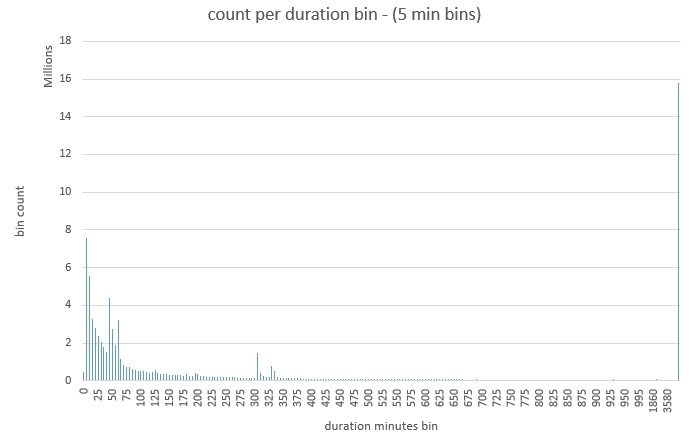
\includegraphics[scale=0.75]{data_session_duration_bin_count.jpg}
	\centering
	\caption[Data session duration distribution]{The single line column bar spike on the right represents sessions of 1 hr duration.}
	\label{fig:data_session_duration_bin_count}
\end{figure}

After we removed the 1 hour duration EDRs newly calculated summary statistics show that the mean and standard deviation decreased to 8 minutes and 14 minutes respectively. This is a 50\% gain with respect to previous statistical data. Further looking at the data session duration frequency plot, by overlaying a cumulative distribution it is shown that 80\% of the records are below the 5 minute mark. These data facts have to be all taken in consideration when assessing the usefulness of the prediction results in evaluation and results in Chapter \ref{chapter:evaluation_and_results}: Evaluation. 



\begin{table}[h]
	\label{table:summary statistics_02}
	\centering
	\resizebox{\textwidth}{!}{
		
		\begin{tabular}{|l|p{5cm}|l|l|}
			\hline 
			\textbf{Summary} & \textbf{timestamp} & \textbf{data session duration (s)} & \textbf{volume (Kb)}\\ 
			\hline  
			count & 82589696 & 82589696 & 82589696\\ 
			\hline 
			mean & null & 458 & 1094048 \\ 
			\hline 
			stddev & null & 827 & 4031503 \\ 
			\hline 
			min & 2016-10-01 00:00:00.000 & 0 & 0 \\ 
			\hline 
			max & 2016-10-31 23:59:59.000 & 3599 &  35590011\\ 
			\hline 
			
	\end{tabular} }
	\caption{Basic summary statistics of main EDR dataset after removing 1 hour duration EDRs.} 
\end{table}

 
 \begin{figure}
 	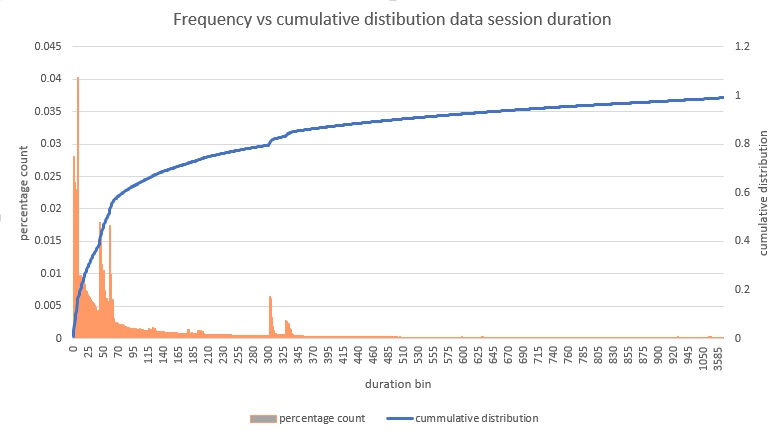
\includegraphics[scale=0.75]{data_session_duration.jpg}
 	\centering
 	\caption[Data session duration cummultive distribution]{80\% of the records are below the 5 minute threshold.}
 	\label{fig:data_session_duration}
 \end{figure}
 


\section{Algorithm Selection} \label{section:methodology:algorithm_selection}

One of the main challenges involved in this study was to assign vehicular traffic to the road network depending on surrounding cell tower traffic in a time series (O\ref{objective:03}).

\subsection{Trajectory interpolation through cell tower data} \label{subsection:methodology:trajectory_interpolation}
We first investigated the possibility to snap the cell tower location data to the road infrastructure mesh depending from which direction the vehicle is coming. Various APIs are available to retrieve nearest road from an input geographical location\footnote{Google Snap to Road API, Bing Map API and OSRM nearest service are examples: https://developers.google.com/maps/documentation/roads/snap (accessed January 8, 2018), https://microsoft.com/en-us/maps/snap-to-road (accessed January 8, 2018), http://project-osrm.org/docs/v5.5.1/api/\#nearest-service (accessed January 8, 2018)}. We investigated how cell tower transmission is configured. There are many settings which determine the range of the cell tower including frequency, rated power, height of tower etc. Given that such information was not available, transmission range of the cell towers was an unknown variable. Another alternative to roughly estimate the range was to calculate the average distance from the nearest \textit{k} neighbouring towers for all cell towers. However from a sample taken from the available dataset of the cell towers across Malta, the variance seemed quite high, ranging from an inter-distance of 150m in urbanized areas to several kilometres in rural areas (comprehensive cell tower locations map across the country not being shown since it is  commercial sensitive information). Furthermore, it was decided to plot the cell towers' on the map and check if their distribution pattern would make it feasible to snap a data record cell tower location to the nearest road or area polygon. Thus here it was assumed that the area around cell towers will have transmission strength with equal range from each tower. Allowance for overlapping was also taken into consideration. 

A typical example of how many road sections there are within an area covered by a number of cell towers can be seen in Figure \ref{fig:cell_towers_distribution}. One can easily appreciate that a lot of roads are associated to a particular cell tower which makes it difficult to devise an algorithm to derive trajectories and traffic flow counts from cell tower location data. Given that there are a lot of unknowns including how handover procedure is handled in specific areas and the actual range of cell towers, the solution path of snapping to nearest roads depending on EDR coordinates was discarded. This approach would have been impractical to assign traffic to junctions, roads or polygon areas and the probability of inaccurate results was high.

\begin{figure}[h]	
	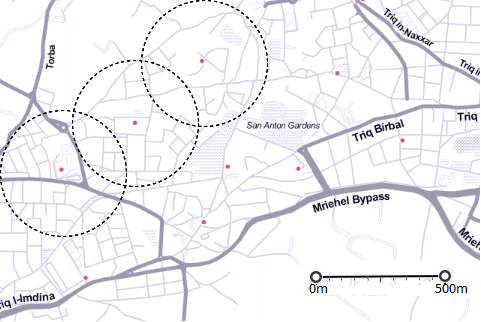
\includegraphics[scale=0.75]{cell_towers_distribution}
	\centering
	\caption[Cell tower distance range]{Cell tower range distribution. Red dots are cell tower locations and dotted line is the estimated range.}
	\label{fig:cell_towers_distribution}
\end{figure}

\subsection{Traffic simulation from OD matrix} \label{subsection:methodology:traffic_simulation_ODMatrix}
Another approach that was considered was to simulate traffic by using statistical information based on travel patterns extracted from the dataset. In Section \ref{section:OD_Matrices} we described how Iqbal et al optimized OD matrices through simulation. An OD matrix can be used as input to a simulation based traffic model. We discuss how an OD matrix was generated in Section \ref{section:methodology:clustering}. 
 
Toledo et al. \cite{Toledo2004} mentions that OD flows are an important input to simulation models but an accurate OD matrix is difficult to acquire. An example of an implementation of a simulation based on an OD matrix can be found in \cite{Hirai2015}. In this study, electronic toll collection data is used to form an initial OD-Matrix. This OD matrix is further improved by optimizing a model that gets observed detector data and a simulation based on current OD, computes the least cost difference and optimizes the OD matrix depending on result. This process is iterated until an acceptable coefficient of determination is achieved. Simulation models generally give two types of outputs namely a visual simulation of traffic flow on a map and textual statistical output that can include metrics such as traffic delays, gap distances, speed and overall trip distance travelled by vehicles.

While macroscopic traffic simulators seem promising for motorways environments they were found to be less suitable for urban scenarios \cite{Bazghandi2012}. Urban environments have a lot of conflicting traffic flows caused by the numerous junctions and small roads that feed and attract traffic from the road network. Also such simulators require accurate OD matrices. This cannot be achieved by using our dataset due to displacement error created by distance separation between cell tower location and actual location.

In our research we tried to focus on both the macroscopic and on the microscopic level since we had a dataset that has ample coverage especially in urban areas.    


\subsection{Traffic flow detection by trip generation assigned\\ traffic} \label{subsection:methodology:trip_generation}
The method we adopted to detect traffic on the road network involved first the generation of an OD matrix that contains main stay locations for users in a time series. Then a trip is generated between each main location for each user as will be explained in Section \ref{section:odmatrix_trip_generation}. The trip includes turn by turn directions with longitude and latitude coordinates. Traffic load assignment is then assigned to junctions and turns depending on the time retrieved from OSM (Open Street Maps) data (see section \ref{section:spatial_binning}). The major challenge here proved to be the traffic assignment, given that there is an interaction of a lot of vehicles at a given point in time with a complex structure of roads and unexpected events such as weather, accidents and road blockages. 


\section{Main activity hubs extraction through clustering} \label{section:methodology:clustering}

One of the main steps of the proposed algorithm is to derive main areas of activity from the mobile data usage of subscribers. This can be achieved using clustering. Clustering was also used to remove noise caused by displacement through frequent oscillations by finding a centroid of activity. The removal of the displacement error through triangulation has been ruled out. There are missing dataset features that are required to get a more accurate location with this process such as strength of signal from every cell tower that the user connects to. Moreover, simple geometrical triangulation does not have the aggregation characteristics that clustering has. Grouping of similar locations have to be implemented on top of triangulation. Triangulation is more suited to remove noise or displacement error caused by cell tower oscillations or handovers. These are caused either because the signal from a tower is weaker from another that can provide better service or there is momentary offloading causing a user to switch his connection to another tower with less load. 

In Section \ref{section:OD_Matrices} it was discussed how certain authors employed various techniques to smooth sudden location change of mobile users because they often switch cell towers in very short time intervals that cannot be attributed to movement. 
 
Clustering is a machine learning unsupervised technique used to classify entities which have similar features. Clustering is done depending on the chosen algorithm and calibration hyper-parameters that control the grouping process. Two clustering techniques that were considered for their appropriateness to this research were k-means and DBSCAN \cite{ChakrabortyNKNagwaniLopamudraDey2011,huang2017research}. 

\subsection{K-means clustering} \label{subsection:methodology:kmeans_clustering}
k-means algorithm is highly popular especially for first analysis of datasets because it is simple to implement and highly efficient. The main drawback of k-means clustering is the requirement to select the number of clusters before running the algorithm. Then a number of expected centroids equal to the number of targeted clusters are randomly chosen. The algorithm starts to find the nearest neighbours based on a distance metric until finally the clusters are formed. This process can be run iteratively until the ideal set of centroids with the least root mean square error are found. Also something important to note is that clusters tend to be spherical in nature. This would be highly visible if 2D clusters are plotted on a graph. The only advantage of using k-means clustering over using DBSCAN is its speed. k-means performs better than DBSCAN especially for incremental version of the algorithms when datasets are frequently updated \cite{ChakrabortyNKNagwaniLopamudraDey2011}.

\subsection{DBSCAN clustering}  \label{subsection:methodology:dbscan_clustering}
DBSCAN (density based spatial clustering of applications) has an edge on k-means and is mostly suited to our research since it does not need to set the number of clusters that we are after for each user at the outset. Moreover it finds clusters of non-spherical nature and leaves noisy elements out of the computed clusters \cite{ChakrabortyNKNagwaniLopamudraDey2011}. DBSCAN has three main hyper parameters to set namely minimum points,  $\epsilon$ (radius of area within which density is measured)  and a distance metric. The algorithm is more sensitive to density rather than to aggregate distance of surrounding points. Basically the algorithm finds core points that have the required minimum points in its neighbourhood dictated by the distance metric. Other non core points that are within core points' radius range (i.e. they are not surrounded with the minimum number of points) are referred to as boundary points. If clusters formed by the core points overlap each other they are grouped together into one single cluster, hence the non-spherical shape of the clusters.


\begin{figure}[!]	
	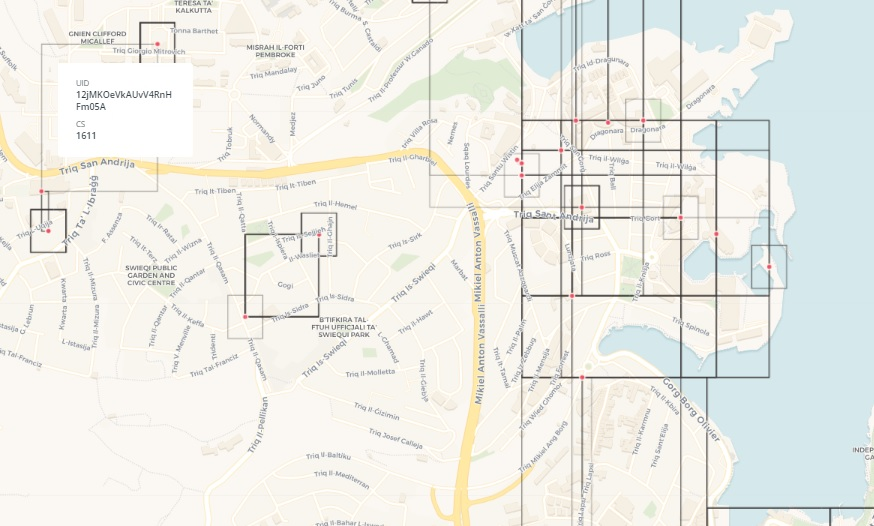
\includegraphics[scale=0.60]{clustering.jpg}
	\centering
	\caption[DBSCAN clustering]{DBSCAN clustering to find main user activity hubs. (Sample illustration)}
	\label{fig:db_scan_clustering}
\end{figure}
 

DBSCAN was the preferred candidate for clustering since the aim was to find dense clusters of mobile data usage activity and random locations visited by users are of no interest and need to be filtered out. The curse of dimensionality does not apply here since there are only two dimensions with the same scale.  The values of hyper-parameters were 500m for radius, minimum required points was set to 3 and euclidean distance was chosen as the distance metric. The mean distance between a sample of cell tower locations taken randomly from the whole dataset was calculated to be 350m. The radius was chosen to be 500m to allow for overlapping but not include too many cell towers accept for the shouldering ones. By choosing an excessive $\epsilon$ the centroid location coordinates was being too inaccurate and was clustering a wide range of subscribers' activity. With a smaller $\epsilon$ minimal clustering (every cell tower will be start to be considered a cluster) was being attained since cell tower location areas will not overlap. 

The OPTICS algorithm, which does away with the $\epsilon$ parameter, iterates until it finds the optimal $\epsilon$ and orders its clusters in a hierarchical result. However this algorithm is more computationally expensive and we opted to use the non-generalized DBSCAN version of the algorithm. The implementation used\footnote{https://github.com/scalanlp/nak (accessed November 10, 2017)} was integrated into Apache Spark processes that output clusters of usage patterns for every user. The output of the implementation we used was in the form of coordinates that outlined the rectangular boundaries of the cluster. The final geographic coordinates that denote the main activity clusters were those of the centroid. The centroid for each rectangular cluster had to be determined with readily available libraries (esri was the used library)\footnote{https://github.com/Esri/spatial-framework-for-hadoop, https://github.com/Esri/geometry-api-java (accessed December 10, 2017)} within Apache Hive. 

In Figure \ref{fig:db_scan_clustering} clustering of cell towers can be observed. The centre of the quadrilaterals would mark the centre of activity for the mobile usage. When there are no cell towers nearby the coordinates of the cell tower itself becomes the centre of activity for the mobile data usage. 



\section{OD Matrix trip Generation}  \label{section:odmatrix_trip_generation}

OD matrix trip generation consists of a sequence of steps. A high-level overview is given in the form of pseudo-code in Algorithm \ref{algorithm:overview}. The main modules of the algorithm will be discussed in detail in the following subsections.
 
\subsection{OD Matrix computation}   \label{subsection:odmatrix_computation}
In our research we decided to focus on two main areas of activity per user as the basis of our OD matrix generation, namely home and work location. Inclusion of more areas of activity is left for future studies (refer to Section \ref{section:future_improvements}). It is assumed that most of the trips happen between home and work and vice versa. This is based on conclusions encountered in related literature (see Section \ref{section:OD_Matrices}). 
The top two mobile data usage activity clusters per user were retrieved from the resulting users' clusters created with DBSCAN algorithm run (see Section \ref{section:methodology:clustering}). We considered these top two clusters as the origin and destination of trips including returns. Then the user EDRs that have geographical coordinates located in the two main activity cluster areas are filtered into a new dataset through the spatial join technique \cite{eldawy2015spatialhadoop}. This process results in a dataset containing all data usage records that have a location in either of the top two clusters for any user in a times series. This resulting dataset is substantially the OD matrix.


\subsection{Trip generation, route choice and traffic assignment} \label{subsection:trip_generation}

Basic OD matrices, on their own, do not give information on how traffic flow is distributed on the roads because they only represent home and work locations. Therefore we had to further enrich the OD matrix by detecting when trips happen by recording change of user cluster location events. This was achieved by ordering OD matrix entries by user and timestamp. The dataset was then scanned and when location of activity of a given record is found to be different from the previous record, the previous record is tagged as a departure and the current one is set as an arrival. We used Apache Hive's window analytic functions for the computations because it offers an sql-like syntax which we were already familiar with and processing is done on top of Hadoop. This made processing of huge amounts of data faster through parallel, distributed computing\footnote{https://cwiki.apache.org/confluence/display/Hive/LanguageManual+WindowingAndAnalytics (accessed February 15, 2018)}. Hive is a data warehouse infrastucture tool running on Hadoop that abstracts a lot of java api calls to get data from distributed file systems managed by Hadoop \footnote{https://en.wikipedia.org/wiki/Apache\_Hive (accessed November 20, 2017)}. Hive has a specific SQL dialect HiveQL(HQL) that can retrieve data from hdfs (hadoop disributed file system) without implementing the mapreduce calls.


There is a caveat on the accuracy of the actual duration of the trip. Records of mobile data usage are generated depending on actual usage at a given location. The frequency of generation of such records has a direct effect on the accuracy of departure and arrival times for any given trip. The higher is the temporal resolution, the more accurate are the departure and arrival times. If on the other hand records are generated at a lower frequency it cannot be determined with confidence and with a low margin of error. For example the user might arrive at his work location but he takes too much time to start his first mobile data session. This would add extra trip delay with the result that the trip duration is less accurate depending on the gap of time between the actual arrival time and the first generated mobile usage record timestamp. Therefore users with more frequent usage of mobile data have trips with durations with a narrower error margin. Departure times are more precise since these are computed by adjusting the EDR timestamp and adding the data session duration. This gives an accurate timestamp that represents when users leave their main clusters (home or work location).   

We inferred the routes between origins and destination from the OSM in a similar manner to the work of Toole et al \cite{Toole2015}. A route was assigned for each entry in the OD matrix together with duration information from the trip. The user's routing choice was assumed to be the fastest one given by the Open Source Routing Machine\footnote{http://project-osrm.org/docs/v5.15.2/api/\#route-service (accessed January 12, 2018)} (OSRM). The OSRM api provides the possibility to request alternative routes. However in the approach taken the route selection was always considered to be static and user does not change route depending on traffic or due to  unexpected events on the road network such as accidents or blockages caused by various other reasons. The fastest route is attributed to each trip done by each user. This may not always be the case since route selection can differ depending on traffic perception and arbitrary route selection made by users. This is a limitation of this research and introduces inevitable bias. It should be noted however that in the urban scenario in Malta the different routes to take towards work and back are limited due to the small scale of the road network infrastructure. In other words there are few possible routes which users can choose from or that enable detouring, making it highly probable that the fastest path is the preferred choice. In Section \ref{section:traffic_flow_evaluation}, it is discussed how to measure a level of confidence in the traffic assignment model.


\begin{figure}[hp]	
	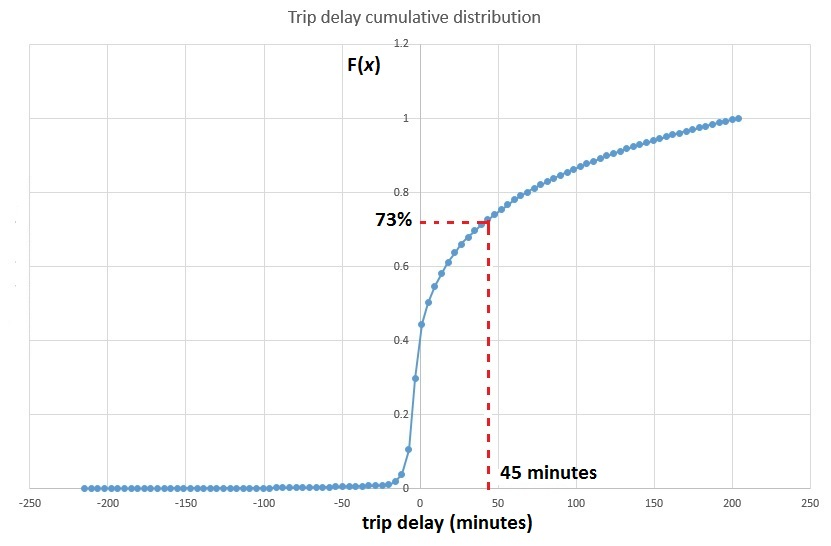
\includegraphics[scale=0.60]{Trip_delay_cumm_distribution.jpg}
	\centering
	\caption[Trip delay cumulative distribution]{Cumulative distribution of trip delay. This figure shows how negative trip delay instances are a very small percentage. Cutoffs  of -5 and 45 minutes were chosen to select the trips for the learning model.  }
	\label{fig:trip_delay_cum_distribution}
\end{figure}

\begin{figure}[!]	
	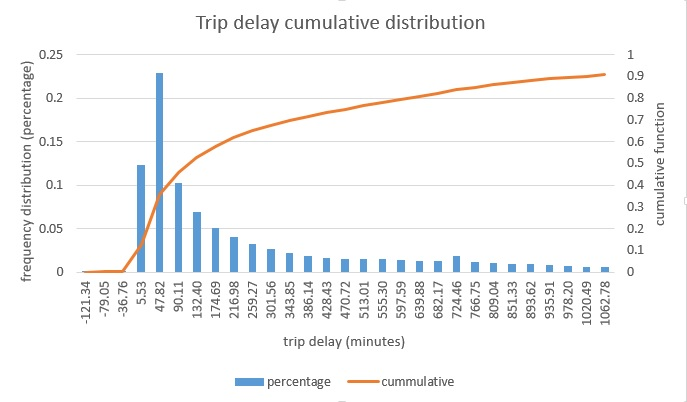
\includegraphics[scale=0.80]{trip_delay_cumm_distribution_total.jpg}
	\centering
	\caption[Trip delay total cumulative distribution]{Trip delay probability distribution presents a heavy tail on the right.  }
	\label{fig:trip_delay_cum_distribution_heavy_tail}
\end{figure}

Another important information that was extracted from the route selection is the trip delay. The total duration for each trip per user was retrieved from the OSRM. The derived route duration does not account for delays. The difference between the actual trip duration retrieved from observed departures and arrivals per user and the OSRM derived trip duration was considered to be the global trip delay. After computing delays for each trip per user, aggregate statistics were collated to describe typical delays at different hours both in weekdays and weekends. Trip delay difference is evident even between Saturdays and Sundays but is highly regular for weekdays as seen in Figure  \ref{fig:trip_delay_weekdays_vs_weekends}. 

A peculiar observation is the negative trip delays. This can be accounted for by actual trips that were faster than expected and estimated by OSRM. Such negative trip delays were observed during the night when people tend to arrive earlier due to almost in-existent traffic. Average trip delay peaks happen between 6:00 a.m. and 7:00 a.m. and 4:00 p.m. and 5:00 pm. for every weekday. Saturdays and Sundays peak trip delays are observed later in the day where usually during weekdays average trip delays are smaller. This can be attributed to the fact that people go out later during the day on these two days. Also, it is clearly noticeable that, for Saturdays and Sundays, only one distinct peak can be seen in the distribution, and average trip delays per hour are much lower in general.

\begin{figure}[h]	
	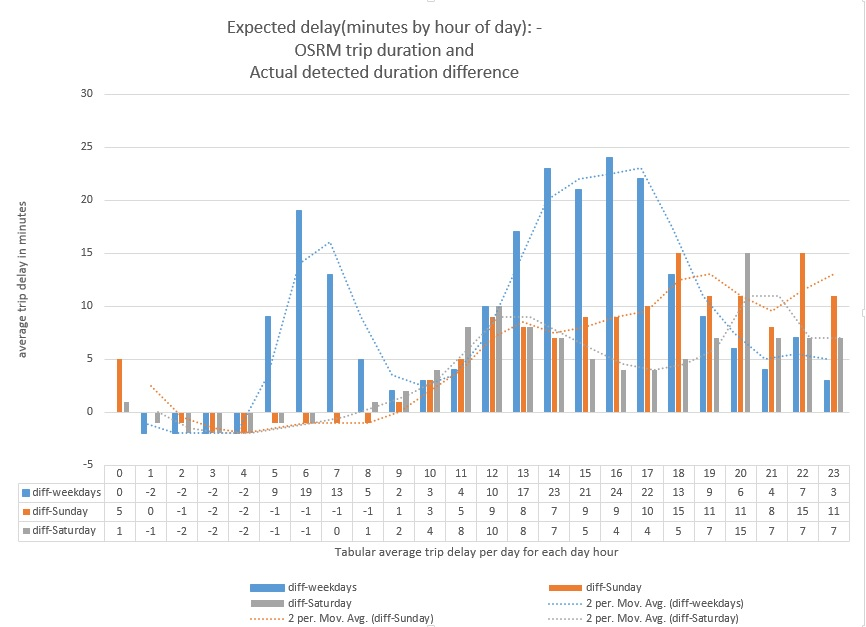
\includegraphics[scale=0.65]{Trip_delay.jpg}
	\centering
	\caption[Hourly average trip delay weekdays vs weekends]{Average trip delay patterns are different between weekdays and weekends. Peaking of average trip delay on weekdays happen between 6:00 a.m and 7:00 a.m. and between 4:00 p.m. and 5:00 p.m. Peaks for weekend days happen later in the day.}
	\label{fig:trip_delay_weekdays_vs_weekends}
\end{figure}

Trip delay data had to be further investigated to remove outliers and data that was not suited for the traffic flow count and the machine learning model had to be filtered out. The data model fitted a heavy tailed distribution as seen in Figure \ref{fig:trip_delay_cum_distribution_heavy_tail}. Data was skewed to the right because of long trip delays attributed to pauses in trips that are likely caused by intermediate location visits between the main areas of activity. Similarly, trip delays of less than -5 minutes\footnote{The negative trip delays are caused by trips with duration less than the one retrieved from the OSRM} were mainly attributed to sudden location displacement caused by cell tower switching (see section \ref{section:OD_Matrices} in chapter \ref{chapter:background} ). Cut-off points were set to -5 minutes and 45 minutes for the lower and upper bounds respectively. Consequently, 50\% of the data was maintained.  

In OSM a route consists of steps and these in turn contain manoeuvres. Manoeuvers encapsulate geographical coordinates data and duration property after which the driving decision should be taken. The manoeuvres' timestamp was computed by accumulating the duration of the previous steps and adding the final total offset to the trip departure timestamp. A new dataset was created with records including previous data structure and steps' information having the timestamp and the coordinates. Therefore, the new dataset, in addition to the coordinates of mobile users at their origin and their destination had trip geolocation information in the form of trip steps.
 

\begin{algorithm}[hp]
	\caption{Experimental Overview}
	\label{algorithm:overview}
	\begin{algorithmic}[1]
		
		\item[]
		
		\BState \emph{\textbf{A. Filter Data}}:
		\Indent	
			\State $\textit{data\_mobile\_usage} \gets \text{filter data usage records from raw \textit{dataset}}$
		\EndIndent
		
		\item[]
		
		\BState \emph{\textbf{B. Main activity locations clustering}}:
		\Indent
		\State $\textit{data\_users\_clusters} \gets \text{run DBSCAN on \textit{data\_mobile\_usage}}$
		\State $\textit{data\_users\_top\_2\_clusters} \gets \text{filter top two user clusters from \textit{data\_user\_clusters}}$
		\State $\textit{data\_users\_top\_2\_clusters\_geo\_data\_points} \gets
				\text{get \textit{data\_users\_top\_2\_clusters} left spatial join \textit{data\_mobile\_usage}}$						
		\EndIndent
		
		\item[]
		
		\BState \emph{\textbf{C. OD Matrix generation}}:
		\Indent
		\State $\textit{data\_users\_top\_2\_clusters\_geo\_data\_points\_sorted} \gets \text{sort by user and datetime } \textit{data\_users\_top\_2\_clusters\_geo\_data\_points}$
		\For{\textbf{each} user group \textit{ug} in $\textit{data\_users\_top\_2\_clusters\_geo\_data\_points\_sorted}$}
			\For{\textbf{each} user record \textit{ur} in \textit{ug}}
				\If {\textit{$ur_t$} cluster id  $\neq$ \textit{$ur_{t-1}$} cluster id (where \textit{t} is timestamp)} 
					\State \textit{$ur_{t-1}$} $\text{departure flag} \gets \text{true}$
					\State \textit{$ur_{t-1}$} $\text{destination coordinates} \gets$ \textit{$ur_t$} $\text{location coordinates}$
					\State \textit{$ur_{t}$} $\text{ actual trip duration} \gets$ \textit{$ur_{t-1}$} $\text{timestamp - }$ \textit{$ur_{t}$} $\text{timestamp}$
				\EndIf
			\EndFor
		\EndFor
		\State $\textit{data\_users\_departures\_arrivals} \gets \text{store final resulting dataset}$
		\EndIndent
		
		\item[]	
		
		\BState \emph{\textbf{D. OD Matrix based trip generation}}:
		\Indent		
			\For{\textbf{each} user departure arrival record \textit{udar} in $\textit{data\_user\_departures\_arrivals}$ }
				\If { \textit{udar departure flag} $=$ true}
				\State $\textit{udar route} \gets \text{derive OSRM route from } \textit{udar origin,destination coordinates}$ 
			
				\State $\textit{udar OSM route duration} \gets  \text{derive OSRM route duration from}$ \par
					\algorithmicindent \textit{udar origin, destination coordinates}
				\State $\textit{udar trip delay} \gets  \text{udar actual trip duration - udar OSM route duration}$						
				
				\EndIf
			\EndFor	
			\State $\textit{data\_users\_trips} \gets \text{store final resulting dataset}$
			\State $\textit{data\_users\_trips\_steps} \gets \text{new empty dataset}$
			
			\For{\textbf{each} user trip record \textit{utr} in \textit{data\_users\_trips} }
		
			    \For{\textbf{each} user trip step \textit{uts} in \textit{utr route}}			    
					\State $\textit{data\_users\_trips\_steps} \gets$ \par
						\hskip\algorithmicindent \text{add new record with step coordinates and timestamp details}
				 
				\EndFor	
			\EndFor			
		\EndIndent			
		
		\item[]
		
		\BState \emph{\textbf{E. Traffic flow spatial binning}}:
		
		\Indent	
	 		
	 		\State $\textit{data\_bin\_traffic\_flow\_time\_series} \gets$ \par 
	 					\text{count traffic flow group by bin id and step timestamp from } \textit{data\_users\_trips\_steps}	
			 	
		\EndIndent		
		
		\algstore{myalg}
			\end{algorithmic}
	\end{algorithm}


\begin{algorithm} [hpt]           
	\begin{algorithmic}[1]           
		\algrestore{myalg}
		
		\BState \emph{\textbf{F. Traffic flow prediction}}:
	    \Indent
		
			\State $\textit{ data\_distinct\_time\_window\_end }  \gets$  $\text{get distinct time window ends from}$ \par
						$\textit{data\_bin\_traffic\_flow\_time\_series}$
			\State $\textit{ data\_distinct\_bin\_ids }  \gets$  $\text{get distinct bin ids from } \textit{data\_bin\_traffic\_flow\_time\_series}$ 
			\State $\textit{ data\_distinct\_time\_window\_ends\_bin\_ids } 	\gets$ $\textit{ data\_distinct\_time\_window\_end } \text{cross join} \textit{ data\_distinct\_bind\_ids }$
			\State $\textit{ data\_sparse\_bin\_count\_time\_series} 	\gets$ \par 
						$\textit{ data\_distinct\_time\_window\_end\_bind\_ids} \text{ left join }  \textit{data\_bin\_traffic\_flow\_time\_series}$ 
			\State $\textit{ data\_time\_windows\_bin\_count} \gets$ \par
			 $\text{two dimensional pivot on } \textit{ data\_sparse\_bin\_count\_time\_series}$ $\text{by bin\_ids}$	
			 
			\State $\textit{ data\_bin\_count} \gets$ $\textit{ data\_time\_windows\_bin\_count}$
			
			
			\State $\textit{ sample\_locations} \gets$ $\textit{ location\_array[a,b,c,d]}$
			\State $\textit{ window\_frames} \gets$ $\textit{ window\_frames\_array[30 min,60 min,180 min,1 day]}$
			
			\item[]
			
			\For{\textbf{each} each bin for location \textit{bin-loc} in  \textit{sample\_locations}}
				\For{\textbf{each} global prediction at \textit{t-ahead} time ahead in \textit{window\_frames}}
					\For{\textbf{each} each record with bin counts \textit{bin-count-record}  for time \textit{t} in \textit{ data\_bin\_count}}						
						\State $\textit{ t-ahead-bin-loc-count} \gets$ $ \text{get bin count for }\textit{ bin-loc } \text{at time} \textit{ t-ahead}$	
						\State $\textit{bin-count-record-with-label} \gets$ \par $ \text{attach} \textit{ t-ahead-bin-loc-count}  \text{ to } \textit{bin-count-record}$				
					\EndFor
				\EndFor
			\EndFor
			
			\item[]
			
			\State $\textit{data\_labelled\_points} \gets \text{store final resulting dataset}$
			
			\State $\textit{ data\_labelled\_points\_reduced} \gets$ \par 
					take first 1000 components of PCA dimensionality reduction of \par 
					\textit{ data\_labelled\_points}
			
			\State $\textit{data\_training} 	\gets$  $ \text{split } \textit{data\_labelled\_points\_reduced} \text{ and get 60\% of data }$
			\State $\textit{data\_testing} 	    \gets$  $ \text{split } \textit{data\_labelled\_points\_reduced} \text{ and get 40\% of data }$
			
			\State $\textit{multilayer\_perceptron\_classifier\_model} 	\gets$  $\text{fit model on } \textit{ data\_training}$	
			\State $\textit{multilayer\_perceptron\_classifier\_prediction\_result} 	\gets$  $\text{run model on } \textit{ data\_testing}$	
			\State \text{report result metrics}
					
			
		\EndIndent 			

	\end{algorithmic}
\end{algorithm}




\section{Traffic flow aggregation through spatial binning} \label{section:spatial_binning}

To get aggregate statistics on traffic distribution, hadoop spatial binning was used as proposed in Eldawy et al \cite{eldawy2015spatialhadoop}. Spatial Hadoop was used due to its highly efficient processing of geolocation data because it uses MapReduce \footnote{https://hortonworks.com/apache/mapreduce (accessed January 20, 2018)} and a 2-level spatial index. MapReduce executes tasks with a level of parallelism and computation is distributed. Spatial Hadoop uses a special algorithm to partition data in Hadoop and maintains a spatial index for fast querying and fast spatial joins \cite{eldawy2015spatialhadoop}. 

A Hive user defined function (UDF) from esri (esri is the company that owns the ArcGIS solution) is used within the Hive query language (HQL) syntax to interact with Hadoop and count traffic flow by spatial bin\footnote{https://github.com/Esri/spatial-framework-for-hadoop (accessed December 10, 2017)}. A spatial bin is a computational geometry that can be used to numerically describe features in a specific region. In our case we used 0.0005 degrees bins to count traffic flow 'steps' derived from OSM routes. 0.0005 degrees bins approximately equate to 50 by 50 metres bins. We are stating that dimensions are not precise when computing the geometrical bin because dimensions are not strictly universal and vary according to map position. These tend to be more of an elongated rectangle near the poles and squarish near the equator. This happens because latitudes get narrower for bins near the poles due to the fact that the earth is not a perfect sphere but an oblate spheroid\footnote{http://www.longitudestore.com/how-big-is-one-gps-degree.html (accessed December 12, 2017)}. Not withstanding this, the bins in the spatial area under investigation are of the same size since Malta does not cover a wide area. We chose $50m^2$ spatial bins to aggregate traffic flow data. In this way we do not have too much wide geometries that can aggregate traffic coming from two roads. Bins with sizes that are less than $50m^2$ make aggregations less meaningful since aggregation is more near to data points rather than grouping polygons. 

\begin{figure}[!]	
	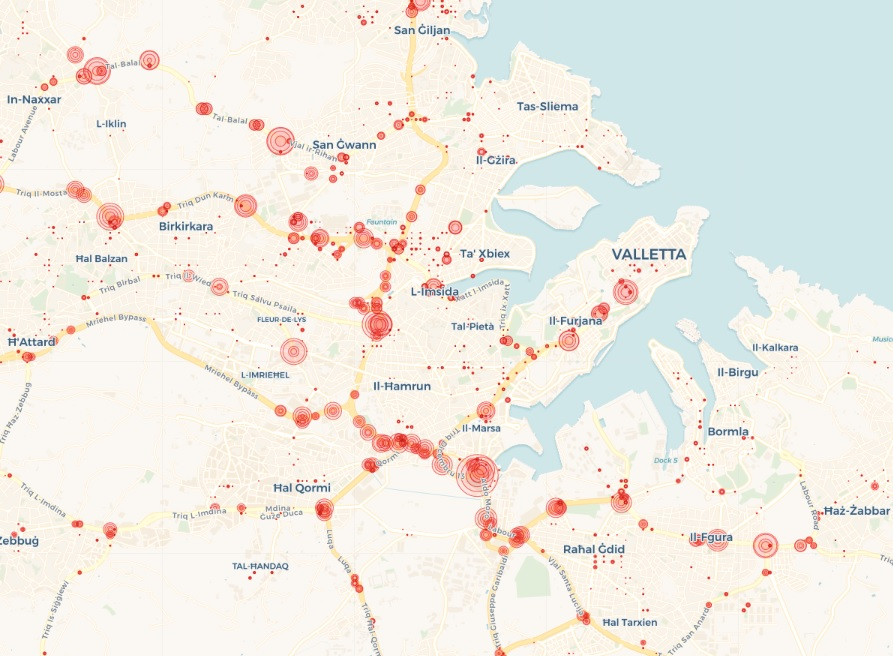
\includegraphics[scale=0.6]{concentric_map.jpg}
	\centering
	\caption{Traffic flow count through spatial and temporal binning. }
	\label{fig:spatial_binning_traffic_count}
\end{figure}

The centroid for each bin was calculated in order to attain the central coordinates of the polygon delineating the bin. Aggregation was not only done spatially but also temporally with intervals of 5 minutes each. This choice of interval's size is quite subjective in nature but it has been decided that it is both granular enough and not too wide to describe traffic flow temporally.  The choice of time ahead window sizes would affect the prediction results. A larger time window would not permit finer prediction in a time series. For example a non-sliding 10 minute time window would allow predictions 10 minutes ahead and a 20 minute sliding window would allow for predictions 20 minutes ahead and so on.

\begin{figure}[!]	
	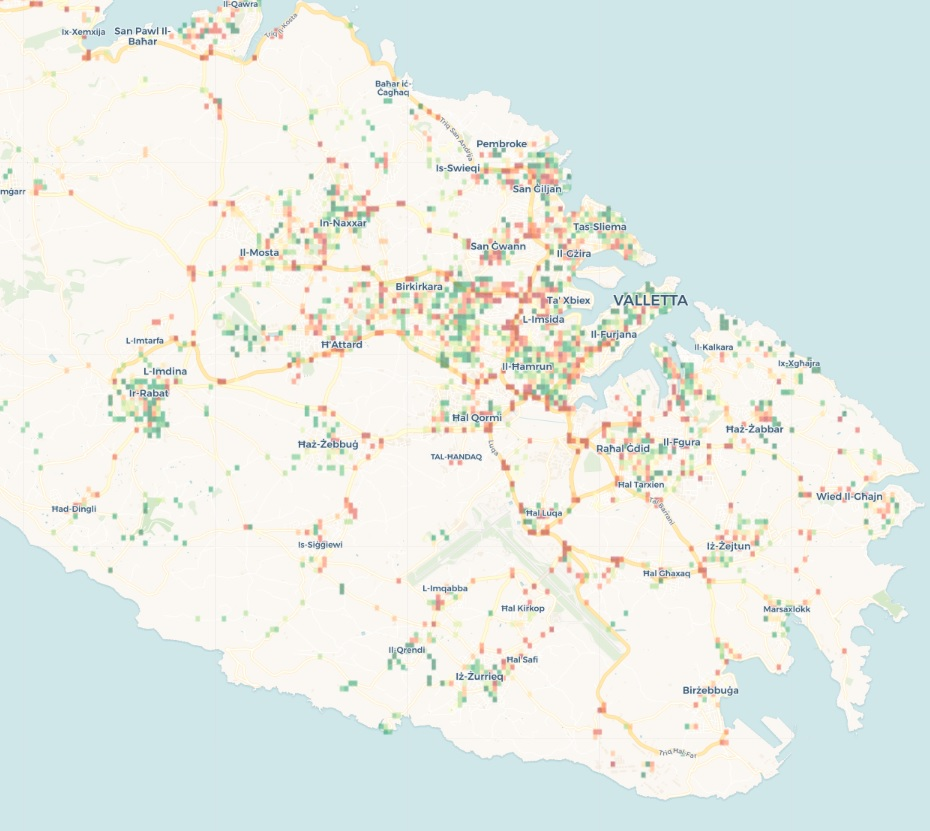
\includegraphics[scale=0.5]{traffic_count_color_coded_categorization.jpg}
	\centering
	\caption[Traffic total flow count binning]{Traffic flow count categorization through a colour coding. Traffic flow count intensity is represented with a colour scheme ranging from dark green (low recorded traffic) to dark red (heavy traffic). The range stretches on 11 quantiles.}
	\label{fig:traffic_count_color_coded_categorization}
\end{figure}

We did not use a sliding window since this would have resulted in less data points for training since training of neural networks would be more costly in terms of computation and would have made analysis more time consuming and complex. Having a sliding window on the other hand makes it more flexible to decouple the averaging window size from the time ahead distance. The prediction time ahead parameter would not need to be a multiple of the averaging window.


Visual tools such as CartoDB\footnote{https://carto.com (accessed May 10, 2018)} where used to illustrate aggregation of traffic flow count in spatial bins. Figure \ref{fig:spatial_binning_traffic_count} shows which areas attract most traffic in Malta. Locations such as the Santa Venera tunnels and Southern Harbour area around the four lane roads in Marsa have bigger distinctive spherical markers indicating that these roads are very busy. The tool allows to select specific date and time to analyse traffic temporally. A similar visualization (figure \ref{fig:spatial_binning_traffic_count}) depicts average traffic intensity across the whole month under investigation. CartoDB allowed us to configure pop ups that can display relative information to the bubble such as location coordinates and average month traffic.

\begin{figure}[!]	
	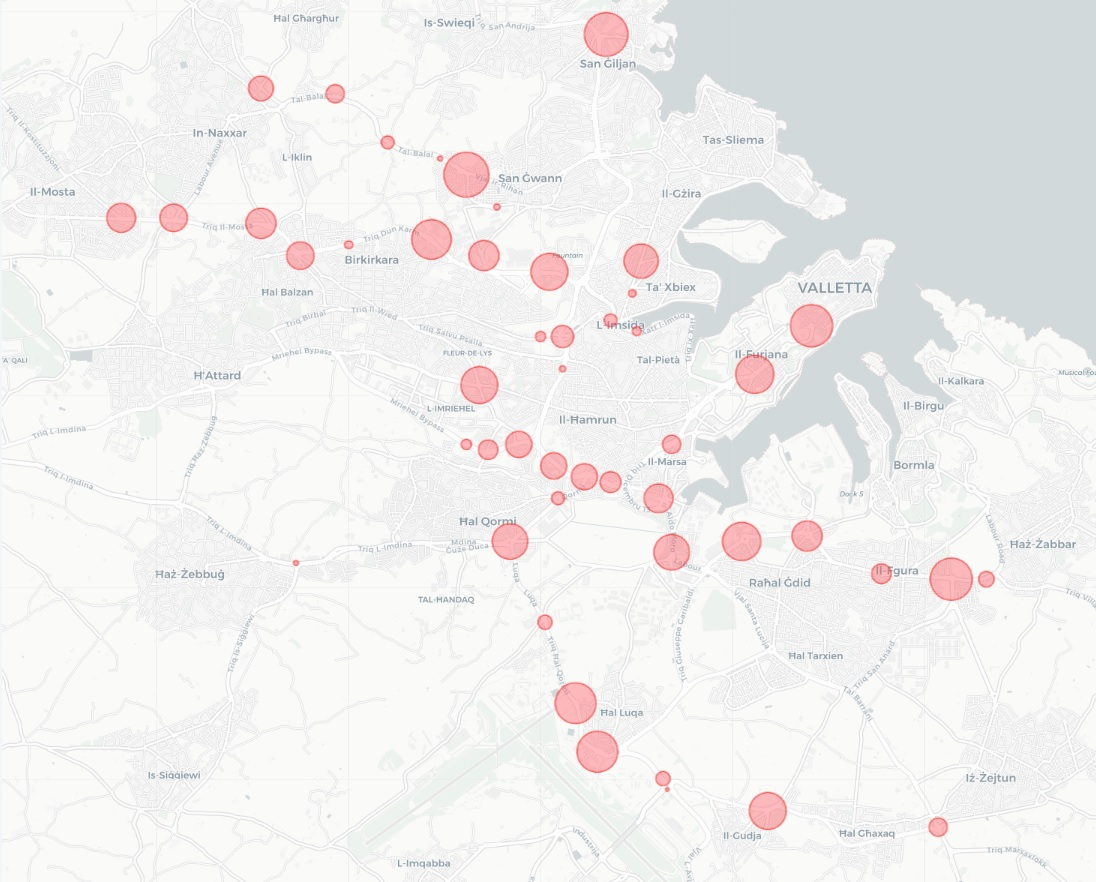
\includegraphics[scale=0.5]{traffic_month_average.jpg}
	\centering
	\caption{Traffic flow count through spatial and temporal binning. }
	\label{fig:traffic_month_average}
\end{figure}

Another illustration (see figure \ref{fig:traffic_count_color_coded_categorization}) uses a colour scheme in a categorical manner to display the intensity of traffic flow. This visualization technique makes it easier to categorize traffic flow count than the technique used to display traffic in figure \ref{fig:spatial_binning_traffic_count}.

CartoDB was a fundamental tool to analyse how traffic flow count changed with time and where. Methods that have been devised in this research to aggregate traffic flow on the road network, can effectively have the generated results illustrated temporally by moving a time window slider in the CartoDB UI. For instance the traffic at 7:00 a.m shown in Figure \ref{fig:traffic_torque_700am} is busier than the traffic at 6:00 a.m. in Figure  \ref{fig:traffic_torque_600am}. Figure \ref{fig:traffic_torque_700am_zoomin} is a zoomed in image of the figure shown in  \ref{fig:traffic_torque_700am}.



\begin{figure}[!]	
	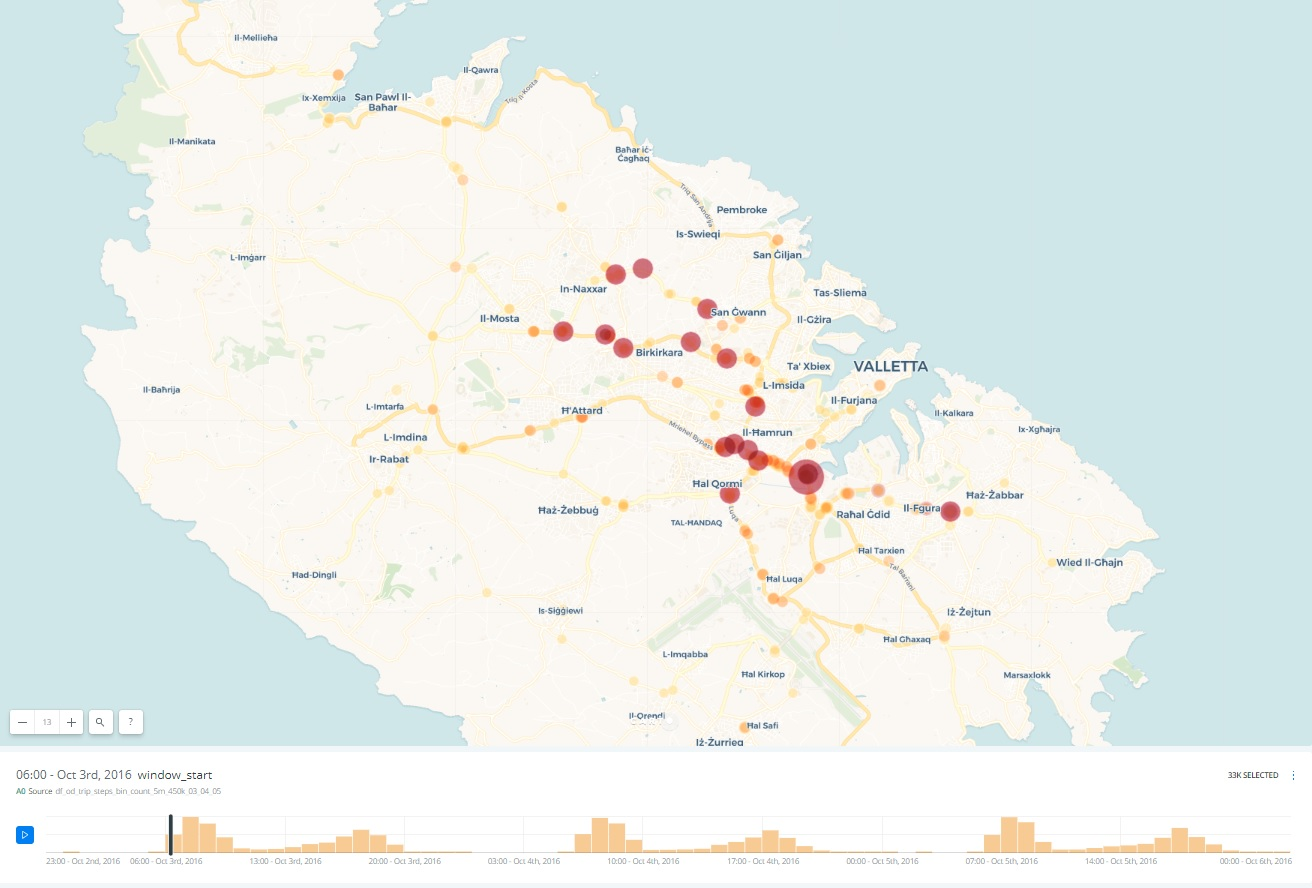
\includegraphics[scale=0.4]{traffic_torque_600am.jpg}
	\centering
	\caption{Traffic flow count at 6:00 a.m. illustrated through CartoDB temporal mapping }
	\label{fig:traffic_torque_600am}
\end{figure}

\begin{figure}[!]	
	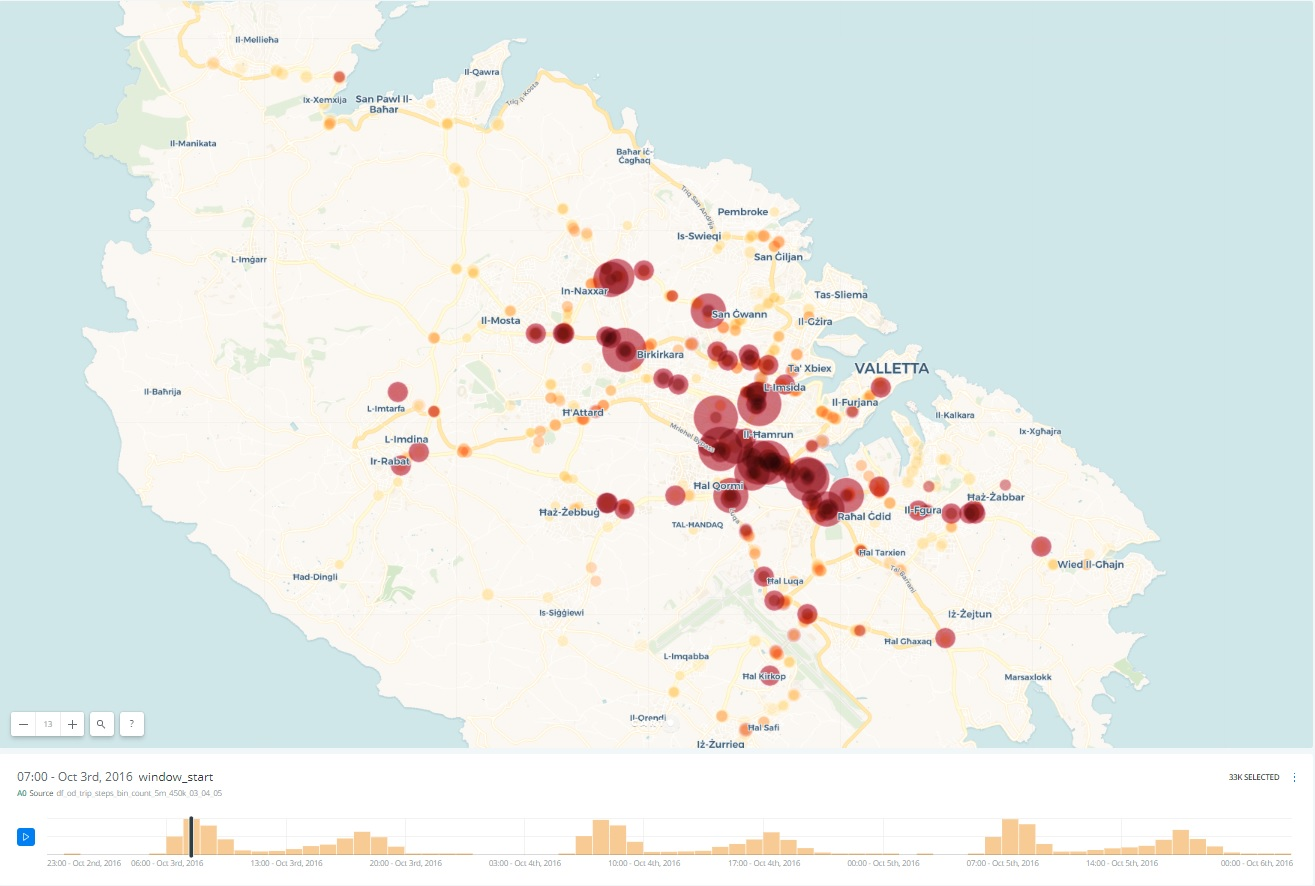
\includegraphics[scale=0.4]{traffic_torque_700am.jpg}
	\centering
	\caption{Traffic flow count at 7:00 a.m. illustrated through CartoDB temporal mapping. }
	\label{fig:traffic_torque_700am}
\end{figure}  

\begin{figure}[!]	
	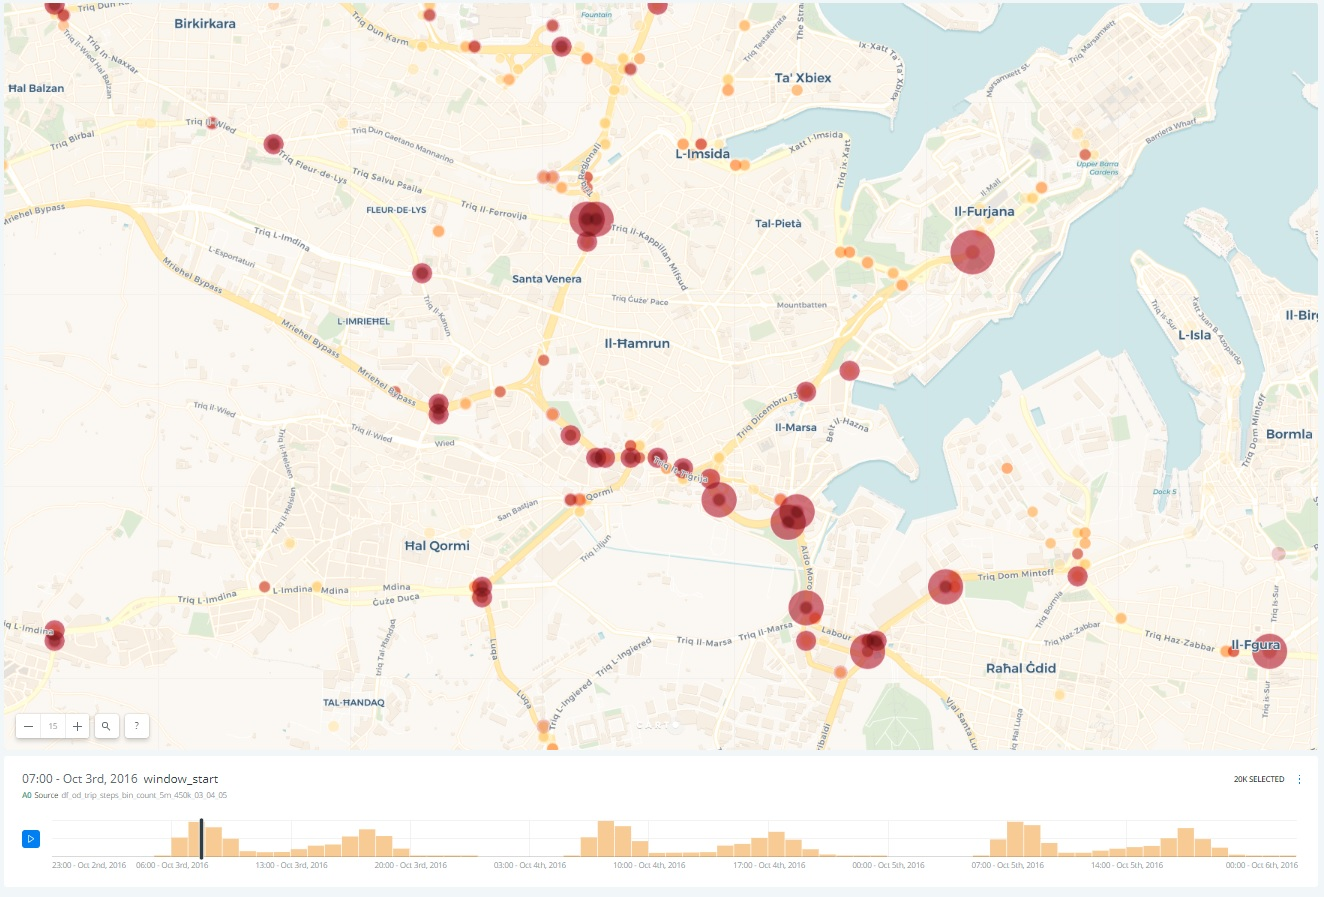
\includegraphics[scale=0.4]{traffic_torque_700am_zoomin.jpg}
	\centering
	\caption{Traffic flow count at 7:00 a.m. illustrated through CartoDB temporal mapping (zoomed in). }
	\label{fig:traffic_torque_700am_zoomin}
\end{figure}

 



\section{Traffic flow modelling and prediction} \label{section:traffic_flow_modelling_and_prediction}


The hypothesis that traffic flow in all areas is directly correlated to how traffic in a specific given area will be in the immediate future determined how the prediction model was structured. More specifically traffic flow at any particular bin $b_i$ at time $t$ influences traffic at bin $b_j$ at time $t + n$. The traffic intensity at any given location is a function of other traffic flow counts from other preceeding bins. The computation of traffic in a location that is based on past traffic cannot be achieved by deriving a mathematical function. A process of artificial intelligence learning is needed in order to build a model. Black box predictive modelling was obtained by training a neural network. Neural networks are known for their ability to generalize and to be able to learn and handle unexpected inputs \cite{sommer2013using}. There were various steps needed to fit a neural network model which was then used to predict the traffic flow. The aim was to select a sample of locations and predict their traffic. In the following subsections, it will be explained how data was processed prior to training of the model, how the model hyperparameters were chosen, how the model was eventually trained and then how the model was validated.

\subsection{Preprocessing data for the prediction model} \label{subsection:Preprocessing data for the prediction model}
The first data mining exercise was to build a dataset where each record contains all Malta traffic flow count for every 5 minutes for the month of October 2016 (see Table \ref{table:dataset_02}). This dataset was then ordered by time. This dataset was to be derived from the generated dataset in Subsection \ref{subsection:trip_generation}. This dataset consisted of aggregated traffic flow for each spatial geolocation in a time series with 5 minutes bins. The final resulting dataset from preprocessing was used to train and validate the artificial neural network (ANN). The features selected to build the model are the traffic flow counts at every location geofenced by a spatial bin. The aggregation process of traffic counts within specific spatial bins was explained in Section \ref{section:spatial_binning}.

We used two configurations for traffic classification. Experimentation with the ANN training and validation was done primarily with four labels. Experimentation was also done with eight labels to test how it would perform in comparison. Classification of traffic was done using 4 labels since traffic is labelled similarly in available traffic applications such as Google Maps Traffic\footnote{https://www.google.com/maps (accessed May 20, 2018)} and Tomtom navigation software\footnote{https://mydrive.tomtom.com (accessed May 20, 2018)}. These labels describe different classes of traffic speed ranging from slow to fast. In Google Maps traffic speed is visualized through colour coding. Green for example is used to indicate slow traffic speeds and dark red is used to notify about heavy traffic congestion.  

In our research Label 1 would indicate very low traffic flow count per minute and Label 4 would represent high traffic flow count per minute. The assigning of the labels consisted first of classifying the traffic count of the bin location for every 5 minute window for which prediction modelling was carried out.  Then the resulting classification was assigned to the $t - 5n$ record where $n$ is an integer denoting the number of fixed time intervals to predict ahead. Therefore after this operation, we introduce another column to Table \ref{table:dataset_03} with future classification of traffic count for a given bin location. 

Four datasets were prepared for training. These datasets were differentiated by the label assigned. The classification label for each dataset record was retrieved from time $t+5n$ ahead through window analytical functions for $n$ with values of 3, 6, 12 and 288.  Since we used a 5 minute binning that sums the traffic flow count, 3,6,12 and 288  time ahead windows would represent 15 minutes, 30 minutes, 1 hour and 1 day ahead predictions respectively.


\begin{table}[h]	
	\centering
	\resizebox{\textwidth}{!}{
		
\begin{tabular}{|l|l|l|l|l|l|}
	\hline 

\textbf{\Large{bin id}} & \textbf{{\Large longitude}} & \textbf{{\Large latitude}} & \textbf{{\Large time window start}} & \textbf{{\Large time window end}} & \textbf{{\Large traffic flow count}} \\ \hline
4611467925420319675 & 14.4320000001052 & 35.905499999918 & 2016-10-01T00:00:00.000Z & 2016-10-01T00:05:00.000Z & 12 \\ \hline
4611467846458306816 & 14.489500000100501 & 35.918499999953397 & 2016-10-01T00:00:00.000Z & 2016-10-01T00:05:00.000Z & 2 \\ \hline
4611468259490374713 & 14.506000000011101 & 35.850499999983199 & 2016-10-01T00:00:00.000Z & 2016-10-01T00:05:00.000Z & 3 \\ \hline
4611468311119383155 & 14.485500000027001 & 35.841999999986903 & 2016-10-01T00:00:00.000Z & 2016-10-01T00:05:00.000Z & 2 \\ \hline

	\hline 
\end{tabular} }
\caption{A sample of traffic flow count by bin for every 5 minute window.} 
\label{table:dataset_02}
\end{table}


The resulting dataset had traffic flow count for each bin with 5 minute temporal resolution. Traffic counts of zero were not yet present before preprocessing. The main features of this dataset included \textit{bin id}, traffic flow count and time window start and end timestamps. 

Further processing was however needed to generate a dataset with records that give a snapshot of all traffic count for Malta for every 5 minutes. First all distinct bin ids where extracted and these amounted to 4134. All the possible time windows of 5 minutes in the month of October were generated, and these amounted to 8928. By performing a Cartesian product between all time series values and all possible bin ids a new dataset with all possible bin id and time window combinations was created. A left join between the original aggregated traffic flow with the latter produced dataset resulted in a new dataset with records that comprehensively describe traffic flow for every 5 minute window for the whole region under study. This data structure was not suitable to be programmatically inputted to the neural network training and further reorganization was necessary. A dataset with data record format where each row contains all traffic flow for all Malta was needed. The columns would be the bin ids that describe all the traffic in all areas. The rows would contain traffic flow count values at a particular 5 minute interval for all these bin ids. To achieve this, a two dimensional pivot was used to transform data and traffic per bin. In the resulting dataset, the traffic count per bin is stored column-wise. The pivot operation based on the data from \ref{table:dataset_02}  resulted in the data that is shown in \ref{table:dataset_03}. 


\begin{table}[h]	
	\centering
	\resizebox{\textwidth}{!}{
		
		\begin{tabular}{|l|l|l|l|l|l|}
			\hline 
			
			\textbf{\large{time window timestamp}} & \textbf{{\large bin id 1}} & \textbf{{\large bin id 2}} & \textbf{{\large bin id 3}} & \textbf{{\large ...}} & \textbf{{\large bin id 4134}} \\ \hline
			2016-10-01T00:00:00.000Z & 0 & 0 & 2 & ... & 0 \\ \hline
			2016-10-01T00:05:00.000Z & 0 & 1 & 1 & ... & 1 \\ \hline
			2016-10-01T00:10:00.000Z & 0 & 0 & 0 & ... & 0 \\ \hline
			2016-10-01T00:15:00.000Z & 1 & 0 & 0 & ... & 0 \\ \hline
			
			\hline 
	\end{tabular} }
	\caption{Sparse traffic flow matrix} 
	\label{table:dataset_03}
\end{table}

After all the feature data were organized in a format that could be fed to the model, a label for each data row was assigned. An ANN is a supervised machine learning type which requires output that can be mapped from input data during the training phase. The output in our case is classification of the level of traffic flow count for a sample location (spatial bin) for which we need to determine the traffic at time $t + 5n$. The output label was not chosen to be the traffic count but the logarithmic function: 

\begin{equation} \label{equation:logarithmic_step_function}
y=\lfloor{log(x+1)/log(max_x/n + 1) * b}\rfloor + 1  \\
\end{equation}

Where $x$ is the actual traffic flow count, $y$ is the final classification label, $n$ is the step size coefficient (the higher it is the smaller the steps)and $b$ is the number of classification levels (bins). 

\begin{figure}[h]	
	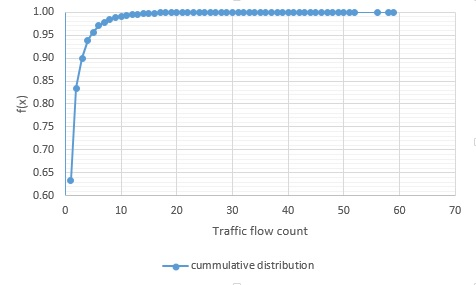
\includegraphics[scale=0.9]{traffic_count_cumm_distribution.jpg}
	\centering
	\caption{Traffic count cumulative distribution for a chosen location. }
	\label{fig:traffic_count_distribution_distribution}
\end{figure}


If a step function with equally spaced intervals was used to classify traffic count, the function label outputs would almost all fall under the first class without meaningful differentiation (see Figure \ref{fig:traffic_count_distribution_distribution}). The skewness towards low counts of traffic is highly decreased with logarithmic binning. The use of logarithmic 'step' function, defined in Equation \ref{equation:logarithmic_step_function}, squeezes indicators in the low traffic flow label bin and widens the range for high level traffic. Note how in Figure \ref{fig:label_classification_of_traffic_count_zoom_in} the logarithmic step function with n=2.36 manages to classify low traffic counts that happen to have high frequency more evenly than step functions with smaller $n$ values. In our experimentation traffic count labelling was done with step size coefficient of 2.36 which proved to give better results for prediction evaluation. Classification of what is easy, moderate or heavy traffic flow is rather subjective. The coefficient of 2.36 value was chosen by changing the coefficient value and visually inspect plots like the one shown in Figure \ref{fig:label_classification_of_traffic_count_zoom_in} to decide that the binning represents proportionally the cumulative distribution of traffic flow count. 

From Figure \ref{fig:label_classification_of_traffic_count_zoom_in} it can be seen that traffic flow count that ranges from 0 to 1 is classified with Label 1 (zero or minimal traffic flow count), traffic flow that ranges from 2 to 3 is classified with Label 2, traffic flow count that ranges from 4 to 10 is classified with Label 3 and traffic flow count that is equal or greater than 11 is classified with bigger labels. More than 60\% of traffic flow count records are classified with Label 1 and more than 20\% are classified as Label 2 traffic flow. 
 
\begin{figure}[!]	
	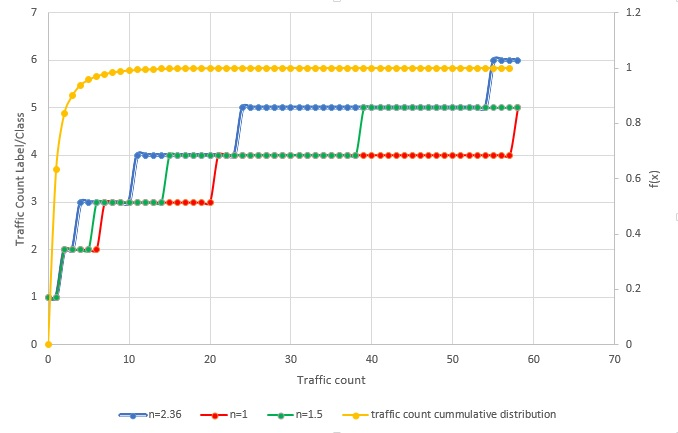
\includegraphics[scale=0.70]{steps_function.jpg}
	\centering
	\caption{Traffic count logarithmic step function. }
	\label{fig:label_classification_of_traffic_count}
\end{figure}

\begin{figure}[!]	
	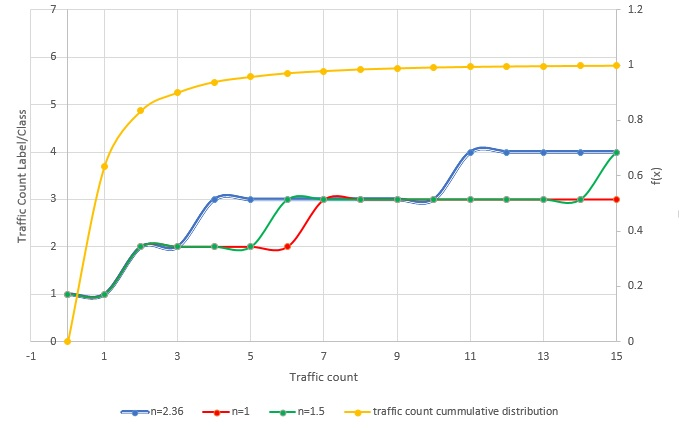
\includegraphics[scale=0.70]{steps_function_zoom_in.jpg}
	\centering
	\caption{Traffic count logarithmic step function showing the lower traffic counts mapping. }
	\label{fig:label_classification_of_traffic_count_zoom_in}
\end{figure}


\subsection{Dimensionality Reduction}
The dataset acquired from the original mobile data usage dataset is huge. The features that describe the data amounted to 4134 as already mentioned in Subsection \ref{subsection:Preprocessing data for the prediction model}. The planned computational complexity depended on how quickly the model converges. However for each iteration carried out to reduce the cost and undergo gradient descent the magnitude of the computations to be performed depended on the number of training examples multiplied by the number of features multiplied by in turn by the number of neurons in each hidden layer. The number of hidden layers was chosen depending on how much complex the problem is but tends to fall victim of overfitting the model if too many layers are inserted in architecture. As mentioned in \cite{Jain1996} ANN design parameters such as number of neurons and number of hidden layers need a trial and error approach to get an architecture that yields better results. Therefore it was important to optimize computation times in order that experimentation that leads to an optimal architecture is less time consuming. Also, the final model is simpler and more practical in terms of getting a prediction after an acceptable amount of time.

\begin{figure}[h]	
	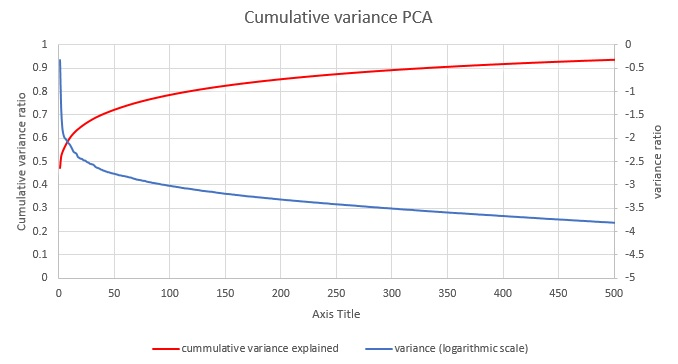
\includegraphics[scale=0.8]{cumulative_variance_pca.jpg}
	\centering
	\caption[PCA first k components cumulative variance]{First components contain a higher percentage of the variance. First 324 components explain 90\% of the variance }
	\label{fig:cumulative_variance_pca}
\end{figure}

One way how to lower computation time was to reduce the number of features. This entails mapping an n-dimensional space to a smaller dimensional space which reduces the number of features in the process. Raschka  \cite{raschka2015python} states that by reducing dimensionality in data there is less risk of overfitting and thus the model can generalize better to testing data.  In \cite{Yang2004} experimentation is done by keeping 95\% and 99\% of the total variance. We chose to keep 324 components that explained 90\% of the total variance. By trial and error it was found that similar results are attained by using 90\% and 98\% of the variance. Original data features showed to be highly correlated, so a high degree of compression was possible through PCA. As explained in the Formula below \ref{equation:principal_components},


\begin{equation} \label{equation:principal_components}
 \mathop{\text{min}}_k \Bigg\{ k : \frac{{\Sigma }_{i=1}^{k} \lambda_i}{{\Sigma }_{i=1}^{n}\lambda_i} \geq r \Bigg\}
\end{equation}

we selected k to be 324 so that the preserved variance ratio $r$ is 90\%. In Equation \ref{equation:principal_components} eigenvalues $\lambda_i$ were ordered in decreasing variance. $n$ represents the original dimensionality of the reduced dataset. In Figure \ref{fig:cumulative_variance_pca}, it can be observed that the first 324 components explain more than 90\% of the data.




\subsection{Prediction through Multilayer Perceptron Classifier}


The next step in the data processing pipeline consisted in predicting traffic from a stipulated time ahead for a given location point. This prediction had to be based on data that was harvested some time before. All of the original datasets had records with timestamps set in the past, so we simulated prediction of traffic flow by trying to forecast traffic at a certain point in time which is ahead of a given timestamp. Evaluation was carried out with a different number of first PCA components, prediction multi-steps ahead and number of possible classes.

As already explained in Subsection \ref{subsection:Preprocessing data for the prediction model}, the multi-step time series prediction was evaluated with a variable amount of steps ahead. Each step was already defined to be 5 minutes long. The experimentation was done with 3,6,12 and 288 steps that reflect 15 minutes, 30 minutes, 1 hour and 1 day. These particular prediction time intervals were selected because practically an individual would need to know traffic in certain locations just before he leaves home. Traffic information 3 hours in advance would prove to be irrelevant for a commuter that just leaves home. This applies especially for Malta based trips, where distances are relatively short and surely any journey is less than 3 hours. Even transport authorities might not find 3 hours beforehand information useful for management purposes. Individual users leaving at 7.00 am in the morning would contribute not information for traffic status at 10.00 am where traffic flow would have eased by then. Therefore we opted to analyse and predict the impact of traffic at 15 minutes, 30 minutes, 1 hour and 1 day before respectively.

One of the first decisions was to choose what type of approach for machine learning to take in order to build a model. The problem at hand was complex, both because of the number of features and the relation they have with each other. A Multilayer Perceptron Classifier (MLPC) is a highly non-linear model that can adapt to problems with high complexity. An MLPC is a specific form of ANN in which perceptrons are feed forward neurons and are interconnected with weights. Layers with a different number of perceptrons define the architecture of the MLP. The first layer is the input layer and the last layer is the output layer. Hidden layers that are optionally inserted in between the input and output layer apply any function to the previous layer and output to the following layer \cite{Jain1996}.

The ANN approach is stated to have the universal approximation property which underlines how an ANN of MLPC type can represent any bounded continuous function to a given arbitrary degree of accuracy \cite{hornik1990universal}. However, it is considered to be a black box that is difficult to control and monitor while learning during the training stage. Spark ML MLPC implementation contains intermediate layer neurons that use the logistic function and output nodes that use softmax function\footnote{https://spark.apache.org/docs/latest/ml-classification-regression.html\#multilayer-perceptron-classifier (accessed April 29, 2018)}.

The Spark 2.3.0 implementation that was used makes use of back-propagation to learn the model. It employs the logistic function as an activation function with Limited-memory Broyden-Fletcher-Goldfarb-Shanno (LBFGS) to minimize error\footnote{https://dzone.com/articles/deep-learning-via-multilayer-perceptron-classifier (accessed May 10, 2018)}.  


The topology choice was determined after carrying out a grid search configured with a set of different hyperparameters. Different configurations for architecture structure were tried out and evaluated until the best performing architecture was chosen. The input and output layers size (number of neurons) are respectively dictated by the number of input PCA extracted features and output classes which are the possible traffic levels indicated by model. Two hidden layers were added to the overall topology. After testing out different possible architectures, the final configuration consisted of 324 neurons for both the input layer and for the second hidden layer, 400 neurons for the first hidden layer and 4 neurons for the output layer which defined the output classes (see Figure \ref{fig:ann_topology}). All architecture layers are fully connected to the successive layer. 


\begin{figure}[!]	
	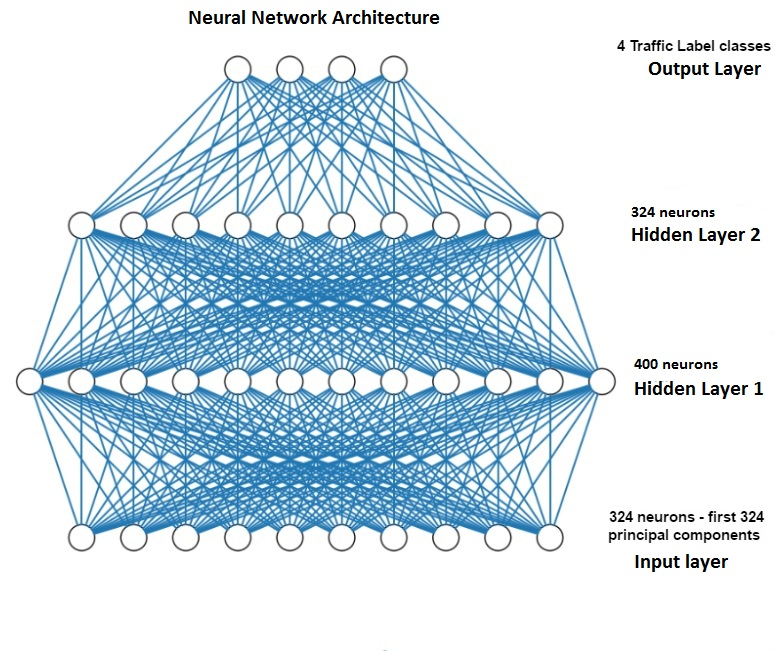
\includegraphics[scale=0.70]{ann_topology.jpg}
	\centering
	\caption[Multilayer Perceptron Classifier topology]{Multilayer Perceptron Classifier topology (324,400,324,4) - generated with python matplotlib library }
	\label{fig:ann_topology}
\end{figure}
 

The available labelled data points dataset was split into 60\% training and 40\% testing. The model with maximum iterations parameter set to 200 showed that after a set of runs it converged consistently. The first phase of setting up the model consisted of the training part where the weights settle to a final value that lead to a minimal error in its classification within the parameter of tolerance set in the configuration. Training outputs a model which is then fitted on the testing data. In the testing phase the prediction efficacy of the model built during training is checked by retrieving certain metrics.



\chapter{Evaluation and Results} \label{chapter:evaluation_and_results}

In this chapter we discuss the systematic evaluation approach that was adopted to get vehicular traffic related information and to build a prediction model from mobile usage data, several stages were involved. The stages in this machine learning pipeline are highly dependent on previous stages' results, mainly, because each stage feeds its output to the next stage. 

Therefore inaccurate results error introduction in early stages would trickle down the pipeline. For example interpretation of error ratio at the prediction stage, which is the last stage, must be primarily  done in the context of results observed in preceding stages. If traffic counts are not accurately measured, the training data itself would not lead to predictions that can be put to practical use. As part of the evaluation process that will be described in detail in the following sections we evaluate four main experimental procedures:

\begin{enumerate}
	\item Average trip counts per hour for weekdays and weekdays
	\item Average trip delay per hour for weekdays and weekends
	\item Traffic flow count in a selection of locations
	\item Traffic count prediction for a selection of locations
\end{enumerate}

%\section{DBSCAN Clustering evaluation}

%Clustering was used to retrieve the top two main mobile usage activity locations for users. Ground truth was not available to test how  accurately the resulting main locations for each user were matching the actual ones. DBSCAN clustering as stated in subsection  \ref{subsection:methodology:dbscan_clustering} detects high density cores and then expands clusters. 

\section{Trip counts per hour evaluation}

After determining the users' daily routes between different origins and destinations two sets of important information were derived. These are namely, trip count and trip delay per route. 

The former represents the average hourly trips done while the latter represents the average delay for every route or for all trips in general. Distributions for both were further derived by using information such as trip departure and arrival timestamp which is available for every route. 

\begin{figure}[!]	
	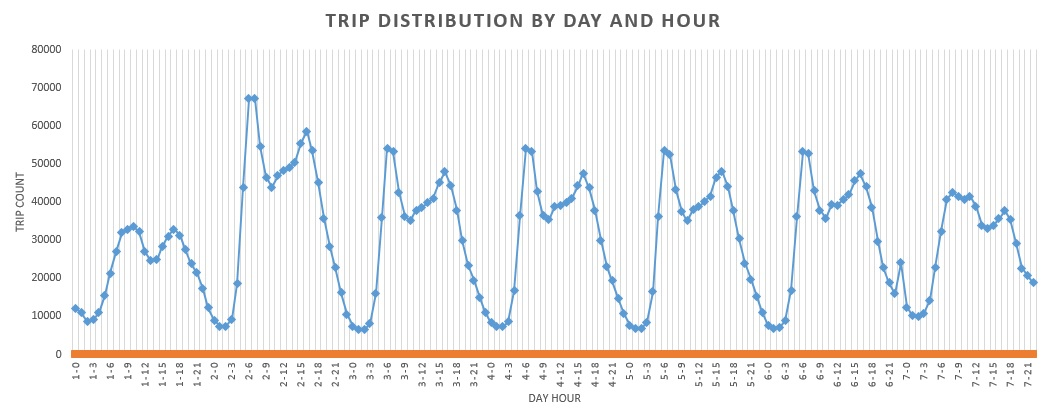
\includegraphics[scale=0.5]{Trip_delay_per_day_week.jpg}
	\centering
	\caption[OD matrix generated trip count]{OD matrix generated trip count patterns per day week. To note how Saturdays and Sundays which are outlined by the last and first two peaks respectively have unique traffic delay patterns.}
	\label{fig:trip_distribution}
\end{figure}


In Figure \ref{fig:trip_distribution}, we show that the trip distribution derived from mobile usage EDRs' generated OD Matrix is strikingly similar with the trip distribution as reported in a National Household Travel survey (NHTS) done in 2010 \cite{malta2011national} (see Figure \ref{fig:trip_distribution_nso}). 


\begin{figure}[!]	
	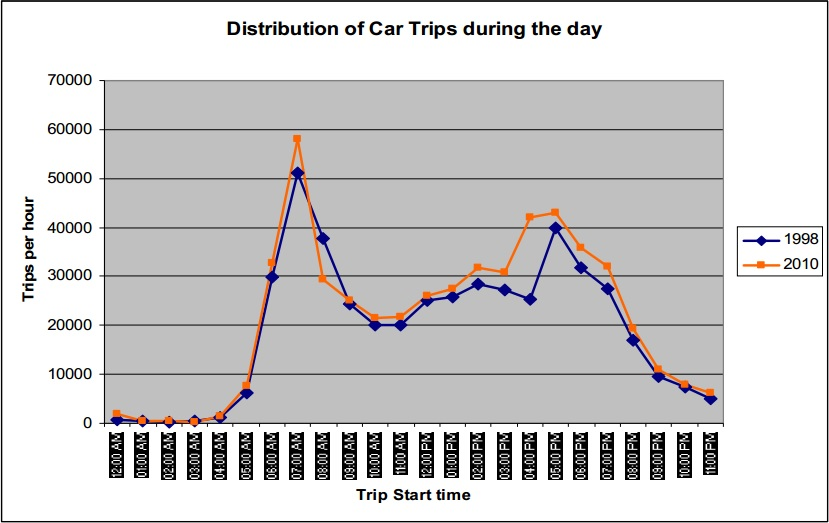
\includegraphics[scale=0.6]{Transport_malta_trip_distribution.jpg}
	\centering
	\caption[NHTS car trip distribution]{Car trip distribution as reported in Transport Malta 2010 National Survey \cite{malta2011national}.}
	\label{fig:trip_distribution_nso}
\end{figure}

As illustrated in figure \ref{fig:trip_count_correlation}, trip count peaks for both reported distributions are observed at 7:00 a.m. and 5:00 p.m. NHTS data was collected on a Wednesday and has no car trip distribution for Saturdays and Sundays. Since figure shown in \ref{fig:trip_distribution} shows that weekdays' OD generated trips count distribution is similar in shape the average was taken on all weekdays of the whole month. However, it should be noted that trip counts on a Monday are distinctively slightly higher than the other weekdays (see figure \ref{fig:trip_distribution}). 


\begin{table}[!] 	
	\centering
	\resizebox{\textwidth}{!}{
		
		\begin{tabular}{|l|l|l|l|l|l|}
			\hline
			\multicolumn{3}{|c|}{\large{\textbf{Linear regression statistics}}}\\
			\hline
			\textbf{Pearson correlation coefficient (r)} & \textbf{ Degrees of freedom} & \textbf{ p-value}  \\ \hline
			0.94 & 22 &  $1.13628e-11^*$ \\ 
			\hline			
			
	\end{tabular} }
	\caption[NHTS and OD trip distributions correlation statistics]{NHTS and OD trip distributions proved to be highly correlated. $ ^* p < 0.001$  } 
	\label{table:trip_dsitribution_statistical_analysis}	
\end{table}

The dynamics of the plot show how there is a sudden decrease of trips per hour after 7:00 a.m. that continues till 11:00 a.m. when trips start to rise again to gradually ramp up. The gradient suddenly increases again at 3:00 p.m. The increase and decrease of trip rate around the 5:00 p.m. peak is smoother than then the one observed in the morning peak for both distributions as shown in Figure \ref{fig:trip_count_correlation}). 


\begin{figure}[!]	
	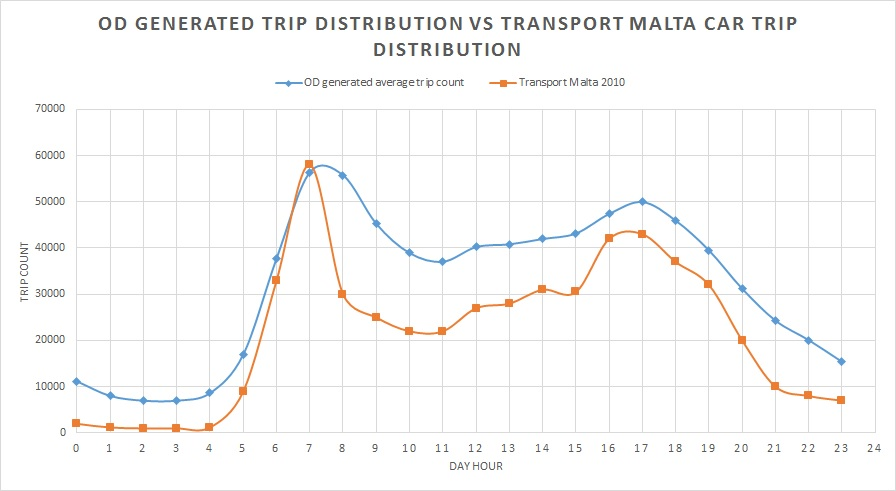
\includegraphics[scale=0.6]{Trip_count_correlation.jpg}
	\centering
	\caption[Comparison between NHTS and OD average trip distribution ]{Comparison between OD average trip distribution over a month and Transport Malta 2010 survey results (\cite{malta2011national})}
	\label{fig:trip_count_correlation}
\end{figure}


NHTS \cite{malta2011national} reports 11\% in car trips from 1998 to 2010 and as shown in Figure \ref{fig:trip_distribution_nso} the distribution again shows resemblance. Both the relationship between HTS datasets gathered in 1998 and 2010 and the relationship of these to the existent OD generated trip dataset demonstrate that trip distribution increases evenly with a specific scale factor across the hours as years go by.


\begin{figure}[!]	
	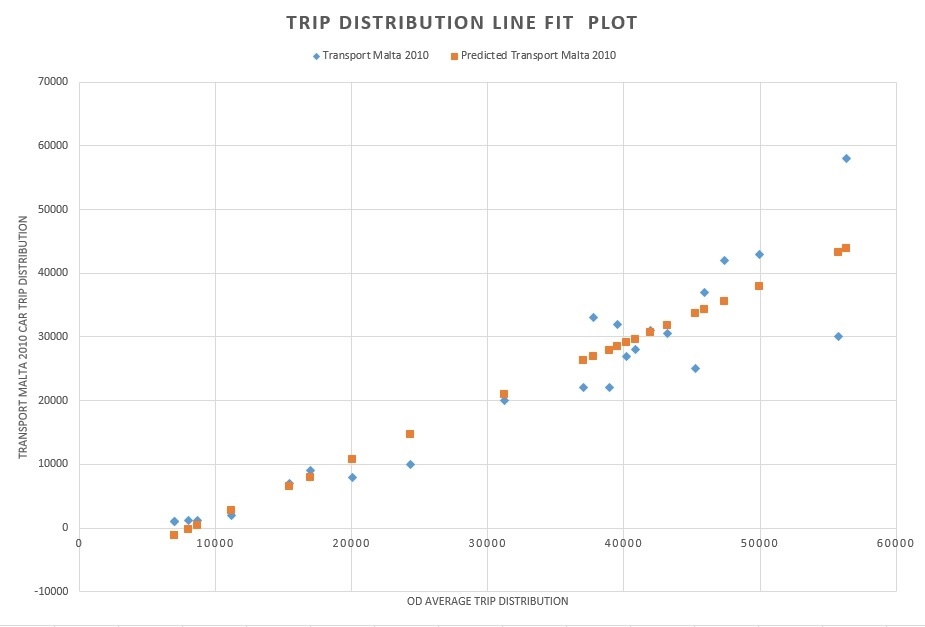
\includegraphics[scale=0.6]{Trip_distribution_line_fit_plot.jpg}
	\centering
	\caption[NHTS and OD average trip distribution linear relationship]{Linear relationship between OD average trip distribution over a month and Transport Malta 2010 survey results \cite{malta2011national}}
	\label{fig:trip_count_correlation_model}
\end{figure}

A linear regression model was devised to express the scaling up from trip distribution in 2010 and the one registered in 2016 in this study. A correlation statistical analysis would have sufficed to establish a linear relationship. There is definitely no causality relationship between these two variables. However, a regression model was fitted to the data to express how scaling up of counts can be done from the OD generated one to actual data that is collected through surveys (see Figure \ref{fig:trip_count_correlation_model}) . Results are reported in Table \ref{table:trip_dsitribution_statistical_analysis} and these show that there is a significant positive relationship between trip distributions.


\section{Trip average delay per hour evaluation} \label{section:trip_average_delay_evaluation}

\begin{figure}[!]	
	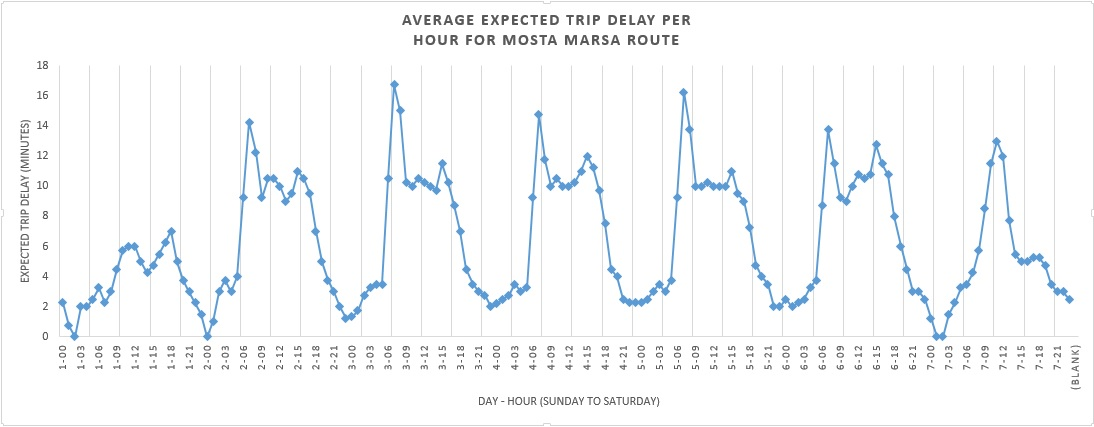
\includegraphics[scale=0.5]{trip_delay_mosta_marsa.jpg}
	\centering
	\caption[Average expected trip delay - 7 day distibution]{Expected trip delay 7 day distribution retrieved with Google distance matrix API for Mosta to Marsa route. Note how Sunday and Saturday delay pattern is different from the one observed for weekdays.}
	\label{fig:trip_delay_mosta_marsa}
\end{figure}

Evaluation of average global trip delay results computed from OD and OSRM generated trips (OD-OSRM) proved to be challenging, because ground truth data could not be found in literature that considered similar research type and in reports from local transport authorities. In the NHTS \cite{malta2011national} in addition to trip count statistics it is mentioned that a detailed matrix with trip information including departure and finish time was compiled. Correspondence with Transport Malta to attain such data or similar information proved to be futile up to the date of completion of this work. 


\begin{figure}[h]	
	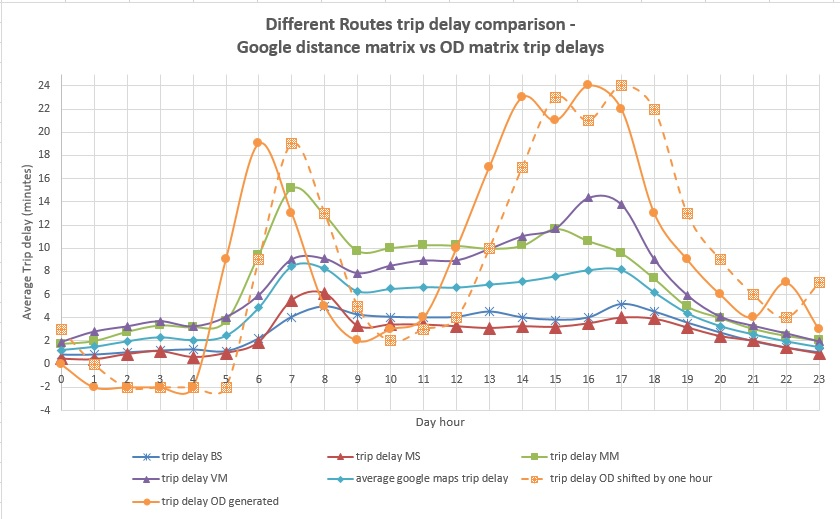
\includegraphics[scale=0.7]{trip_delay_comparison.jpg}
	\centering
	\caption[Trip delay line chart DMAPI vs OD-OSRM]{DMAPI expected average trip delay comparison with OD-OSRM computed average trip delays for routes: Mosta to Marsa (MM), Mellieha to Swieqi (MS), Birkirkara to Sliema (BS), Valletta to Mgarr (VM)}
	\label{fig:trip_delay_google_vs_mine}
\end{figure}


At the end of April 2018 Google maps made available traffic information overlay on its maps. In addition to this Google Cloud distance matrix API  (DMAPI) exposed a web service that gives duration and duration in traffic of trips that are defined with origin and destination for Malta as well.

\begin{table}[!]	
	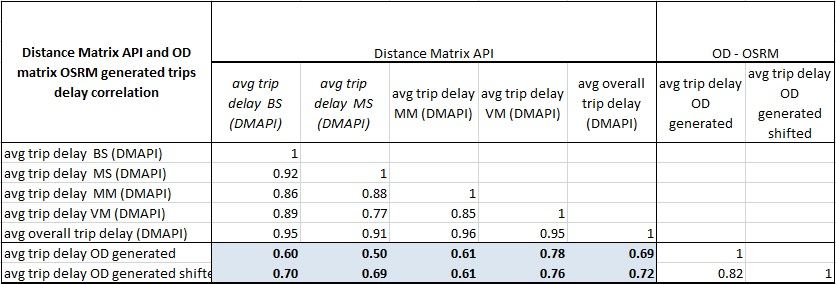
\includegraphics[scale=0.7]{trip_delay_correlation_DMAPI_vs_MINE.jpg}
	\centering
	\caption[Trip delay correlation statistics between DMAPI and OD-OSRM]{Correlation statistics between DMAPI routes' average trip delay and DMAPI routes' correlation with OD-OSRM computed trip delay. Note that correlation is being done between data retrieved in June for DMAPI and data retreived in October for OD-OSRM}
	\label{table:trip_delay_google_vs_mine}
\end{table}


The trip delay model built through the OD matrix is a basic statistical one that gives average trip delay per hour. Google distance metric API gives estimated duration information (with traffic and without) by specific route. In order to compare the estimations of our model with the Google one for the local traffic a data-mining process that scraped a data set of trip delay through the DMAPI web service was carried out. Figures \ref{fig:trip_delay_carto_db} and  \ref{fig:trip_delay_google_900am} show traffic status for the same zone at the same hour for OD-OSRM traffic flow count and Google traffic status. Note the similarity in how traffic hotspots' locations are shown.

\begin{figure}[!]	
	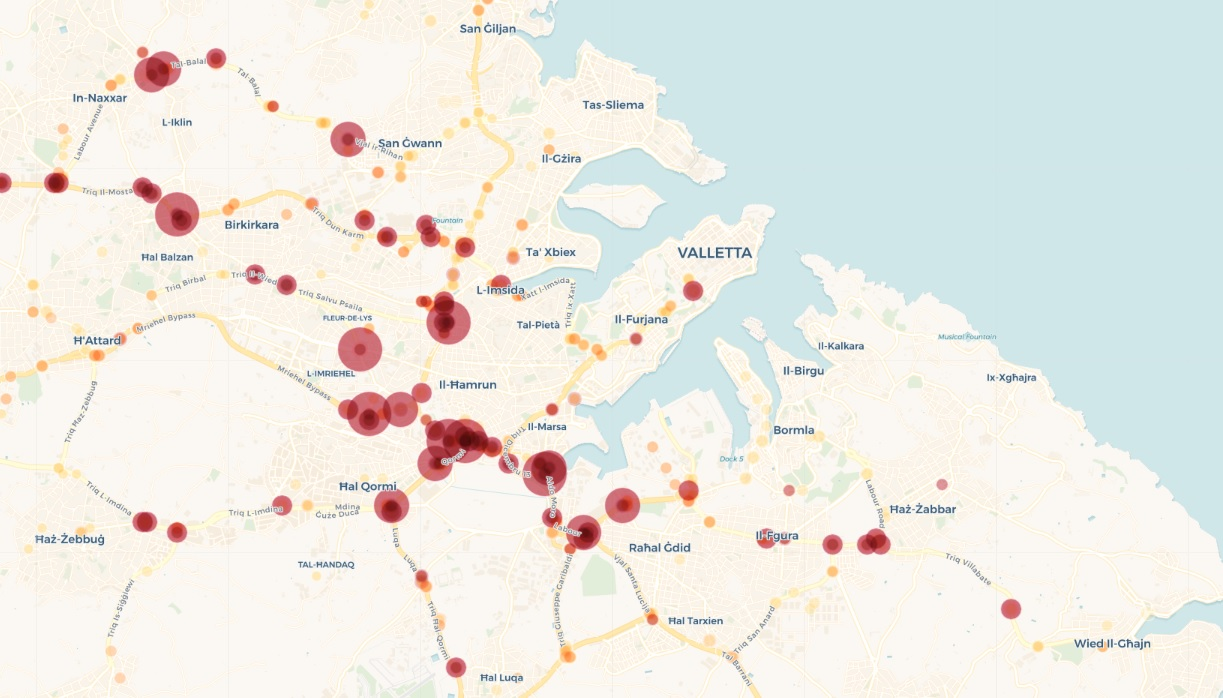
\includegraphics[scale=0.4]{OD-OSRM_traffic_900am.jpg}
	\centering
	\caption[OD-OSRM traffic flow count mapping]{OD-OSRM traffic flow count mapping at 8:00 a.m. on a weekday}
	\label{fig:trip_delay_carto_db}
\end{figure}

\begin{figure}[!]	
	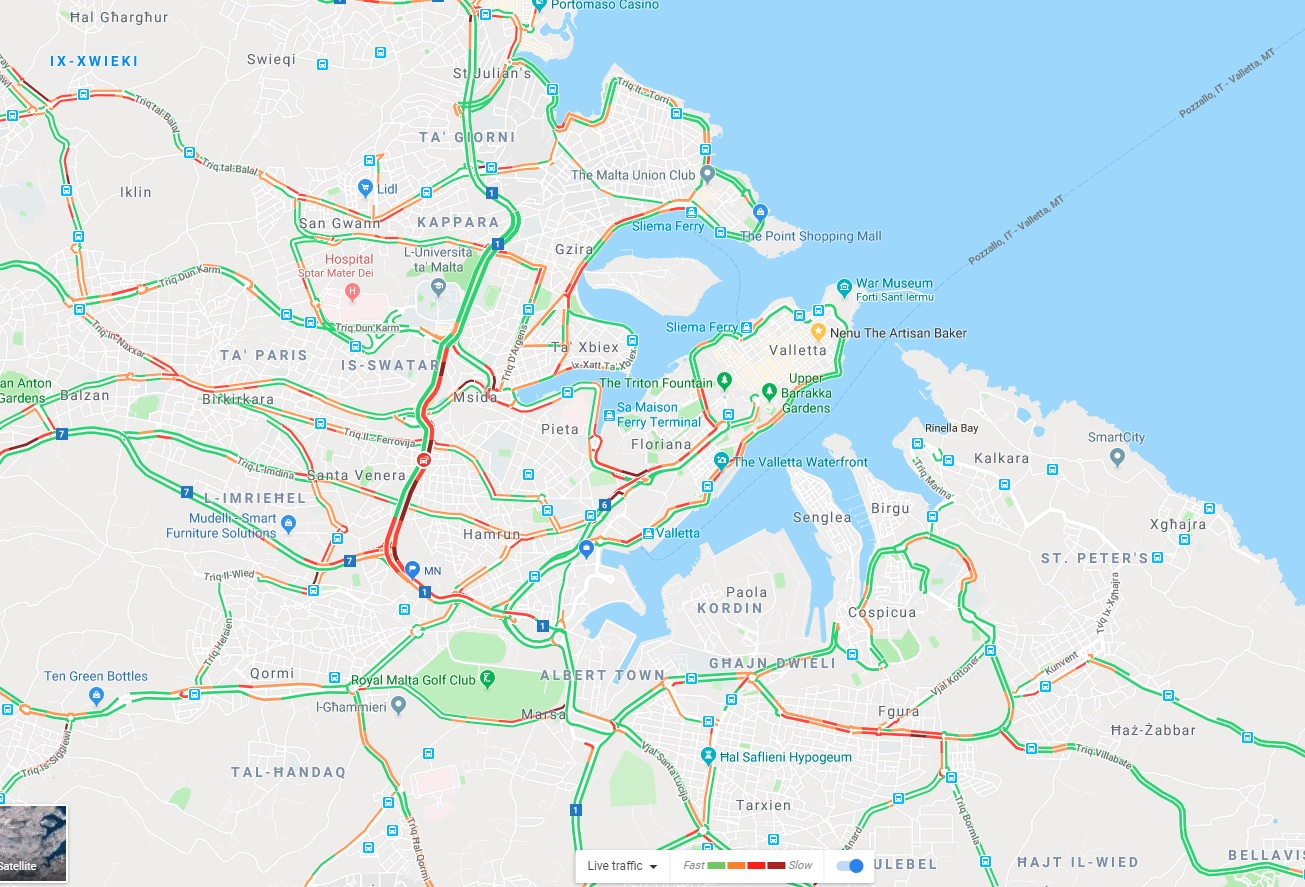
\includegraphics[scale=0.4]{google_traffic_900am.jpg}
	\centering
	\caption[Google Map Traffic delay mapping]{Google Map Traffic mapping at 8:00 a.m. on a weekday - to compare with OD-OSRM traffic flow count mapping}
	\label{fig:trip_delay_google_900am}
\end{figure}
 

Seven whole days of Google DMAPI data from June 2018 was scraped by retrieving duration information for every quarter of an hour (see Figure \ref{fig:trip_delay_mosta_marsa} for an example). Estimated trip delay is calculated by subtracting estimated trip duration from trip duration in traffic. Average trip delay was then computed per hour. This process was done for four different routes namely Mosta to Marsa (MM), Mellieha to Swieqi (MS), Birkirkara to Sliema (BS) and Valletta to Mgarr (VM) and the overall trip delay average was calculated on these routes. These routes were chosen for two reasons. Firstly these were chosen because they represent routes that are really varied in type in terms of direction and areas covered. Secondly because the average time of the selected route trips which is retrieved from Google API (24 minutes) approximates the global trip average time which is reported for a car trip in \cite{malta2011national} (20 minutes). To be noted however that from 2010, trip delays likely increase was due to further loading of traffic on the road infrastructure.

Correlation results showed that there is a strong linear relationship between the routes' trip delay pattern which were investigated with the DMAPI. Correlation between DMAPI and OD-OSRM trip delay estimation is less but still considerable. Between DMAPI average overall trip delay and OD-OSRM non shifted expected trip delay data there is a correlation of 0.69 (see table \ref{table:trip_delay_google_vs_mine}).

When comparing trip expected delays we noticed some distinctive features that differentiate OD-OSRM trip delay plot and the DMAPI ones. Trip delays are higher in OD-OSRM data than for DMAPI. We also noted that patterns for plots based on DMAPI retrieved trip delay data tend to have delays peaking distinctively higher in the morning rather than in the afternoon. Furthermore, OD-OSRM trip delay morning peak comes 1 hour earlier. The fact that more trip delay is observed for the OD-OSRM dataset can be attributed to the fact that in October there is much more traffic. It is known that in Malta, October is one of the most chaotic months for traffic because schools and colleges would have just started. In June, the University of Malta semester is almost closing (no more lectures are being held) and primary and secondary students finish in the early afternoon. Government department work till midday from mid June as well. The earlier peak observed in the OD-OSRM data can be explained in the light that, in October, to cope with the heavy delays on the roads, commuters leave earlier to avoid traffic congestion. When shifting the OD-OSRM data by one hour (see dotted line in fig. \ref{fig:trip_delay_google_vs_mine} ) a higher correlation of 0.78 is observed with (DMAPI) overall average trip delay.

The fact that the data has different seasonality is a serious limitation in the evaluation of the OD-OSRM trip delay model with DMAPI data as ground truth. Given that at the time of writing results could not be recomputed for OD-OSRM for June it was attempted to get DMAPI webservice estimations data for October 2018. DMAPI does not give responses for data queries that request past data. However, it can give expected trip duration data in the future even if is queried from months ahead. The data retrieved for 7 days in October 2018 with DMAPI from four months in advance was exactly the same as the one retrieved for the same route in June. Therefore there was not the possibility to evaluate our model with DMAPI data from the same month which was expected to a have a more similar pattern. Still, from the perspective of knowing how traffic in June and October is different, and the strong correlations between the trip delay estimation models, there is a good confidence level in relying on the OD-OSRM trip delay estimation data.	

\section{Traffic flow count evaluation} \label{section:traffic_flow_evaluation}

Route information was retrieved from OSRM with the OD matrix as input. Thus with a matrix of origins and destinations each trip done by any user was assigned a route (refer to method discussed in Section \ref{subsection:trip_generation}). The fastest route was retrieved from the OSRM and alternative routes were not considered. This is decisive together with OD matrix computation to characterize the traffic assignment model. The average OD-OSRM computed traffic flow count was compared with average actual traffic flow counts at the same locations and at the same exact date and time in order to analyse how accurately the traffic assignment distributes traffic flow with fastest route as default selection.


%---------------------------------- TRAFFIC FLOW COUNT NIGEL PACE VS MINE -------------------
\begin{figure}[!] 
	\centering
	\begin{subfigure}{0.8\textwidth}
		\centering
		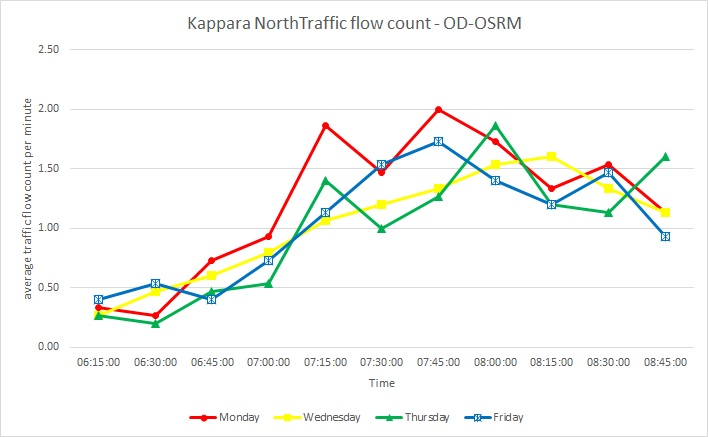
\includegraphics[width=\linewidth]{traffic_flow_count_KN_MINE.jpg} 
		\caption{\scriptsize{Traffic flow Count Kappara North - OD-OSRM}} 
		\label{fig:traffic_flow_count_KN_MINE}
	\end{subfigure}
	
	\vspace{1cm}
	\begin{subfigure}{0.8\textwidth}
		\centering
		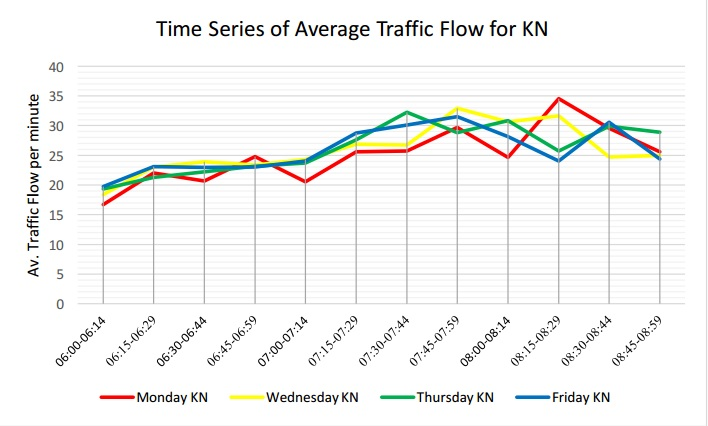
\includegraphics[width=\linewidth]{traffic_flow_count_KN_Nigel_pace.jpg} 
		\caption{\scriptsize{Traffic flow Count Kappara North - video stream count}}
		\label{fig:traffic_flow_count_KN_NP}
	\end{subfigure}
	
	\caption[Kappara North Traffic flow counts from OD-OSRM and video stream count comparison]{Kappara North Traffic flow counts from OD-OSRM and video stream count comparison. Video stream count graphic has been reproduced from \cite{Pace2017}.}
	\label{fig:kappara_north_traffic_flow_line_chart}
\end{figure}

\begin{figure}[!] 
	\centering
	\begin{subfigure}{0.8\textwidth}
		\centering
		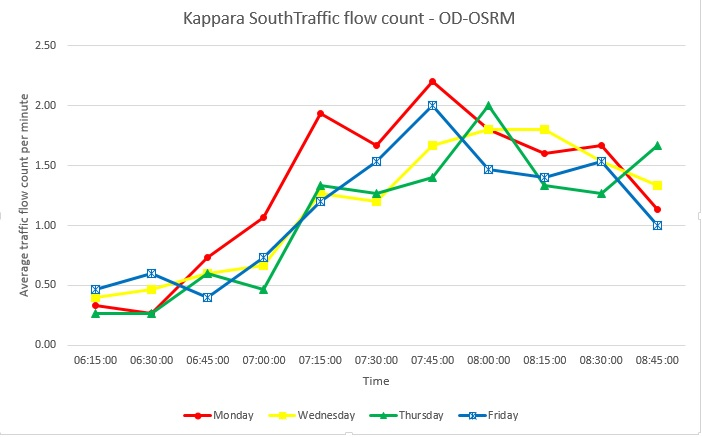
\includegraphics[width=\linewidth]{traffic_flow_count_KS_MINE.jpg} 
		\caption{\scriptsize{Traffic flow Count Kappara South - OD-OSRM}} 
		\label{fig:traffic_flow_count_KS_MINE}
	\end{subfigure}
	
	\vspace{1cm}
	\begin{subfigure}{0.8\textwidth}
		\centering
		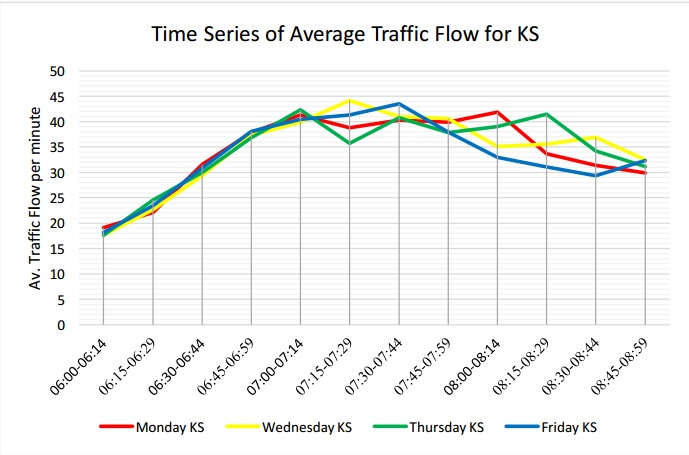
\includegraphics[width=\linewidth]{traffic_flow_count_KS_Nigel_pace.jpg} 
		\caption{\scriptsize{Traffic flow count Kappara South - video stream}}
		\label{fig:traffic_flow_count_KS_NP}
	\end{subfigure}
	\caption[Kappara South Traffic flow counts from OD-OSRM and video stream count comparison]{Kappara South Traffic flow counts from OD-OSRM and video stream count comparison. Video stream count graphic has been reproduced from \cite{Pace2017}}
	\label{fig:kappara_south_traffic_flow_line_chart}
\end{figure}


\begin{figure}[!] 
	\centering
	\begin{subfigure}{0.8\textwidth}
		\centering
		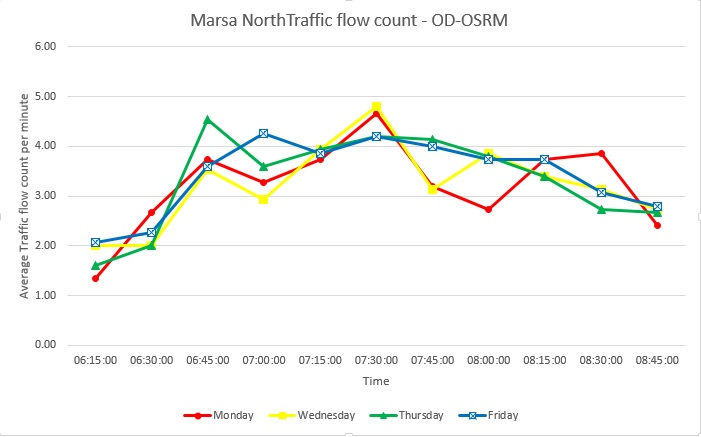
\includegraphics[width=\linewidth]{traffic_flow_count_MN_MINE.jpg} 
		\caption{\scriptsize{Traffic flow count Marsa North - OD-OSRM}} 
		\label{fig:traffic_flow_count_MN_MINE}
	\end{subfigure}
	
	\vspace{1cm}
	\begin{subfigure}{0.8\textwidth}
		\centering
		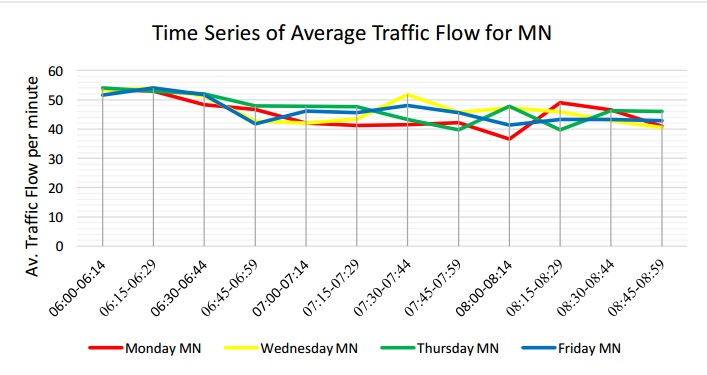
\includegraphics[width=\linewidth]{traffic_flow_count_MN_Nigel_pace.jpg} 
		\caption{\scriptsize{Traffic flow count Marsa North - video stream}}
		\label{fig:traffic_flow_count_MN_NP}
	\end{subfigure}
	\caption[Linear chart for Kappara northbound and southbound traffic flow]{Marsa North Traffic flow counts from OD-OSRM and video stream count comparison. Video stream count graphic has been reproduced from \cite{Pace2017}.}
	\label{fig:marsa_north_traffic_flow_line_chart}
\end{figure}

\begin{figure}[!] 
	\centering
	\begin{subfigure}{0.8\textwidth}
		\centering
		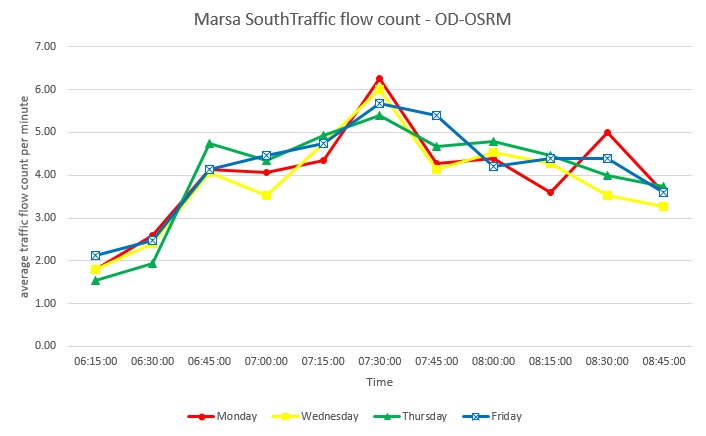
\includegraphics[width=\linewidth]{traffic_flow_count_MS_MINE.jpg} 
		\caption{\scriptsize{Traffic flow count Marsa South - OD-OSRM}} 
		\label{fig:traffic_flow_count_MS_MINE}
	\end{subfigure}
	
	\vspace{1cm}
	\begin{subfigure}{0.8\textwidth}
		\centering
		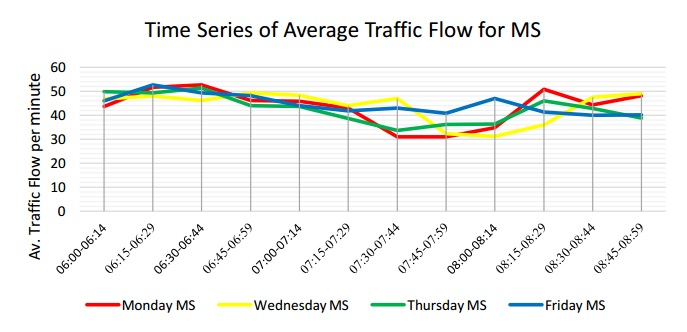
\includegraphics[width=\linewidth]{traffic_flow_count_MS_Nigel_pace.jpg} 
		\caption{\scriptsize{Traffic flow count Marsa South - video stream}}
		\label{fig:traffic_flow_count_MS_NP}
	\end{subfigure}
	
	\caption[Line chart for Marsa northbound and southbound traffic flow]{Marsa South Traffic flow from OD-OSRM and video stream counts comparison. Video stream count graphic has been reproduced from \cite{Pace2017}.}
	\label{fig:marsa_south_traffic_flow_line_chart}
\end{figure}

%-----------------------------------------------------------------------------------------------------

The ground truth data that was used, came from work done by Nigel Pace in his dissertation submitted in 2017 \cite{Pace2017}. Directional traffic flow counts were manually gathered from web camera streams recorded from four locations. These were gathered from Kappara and Marsa roadways for traffic which is both northbound and southbound. The Marsa roadway is referred to as the Marsa-Hamrun bypass, which is the road leading to and from the Santa Venera tunnels. These roads are known for heavy traffic loads and congestion in Malta. The Kappara roadways get and feed traffic to the old Kappara roundabout which today has been replaced by a flyover. The dates for the data collection were from Monday 17th October to Friday 21st October. Data for the day of Tuesday 18th October was missing from the dataset and there was no particular reason specified why this was missing. The traffic flow count consisted of an average traffic flow count per minute taken over intervals of 15 minutes. This resulted into 44 samples for data gathered from 6.00 a.m to 8.45 a.m. for every day. A daily average for every quarter of an hour was then taken for both the actual data and the one generated with OD-OSRM.   


%---------------------------------- TRAFFIC FLOW COUNT LINE PLOTS -------------------

\begin{figure}[!] 
	\centering
	\begin{subfigure}{0.8\textwidth}
		\centering
		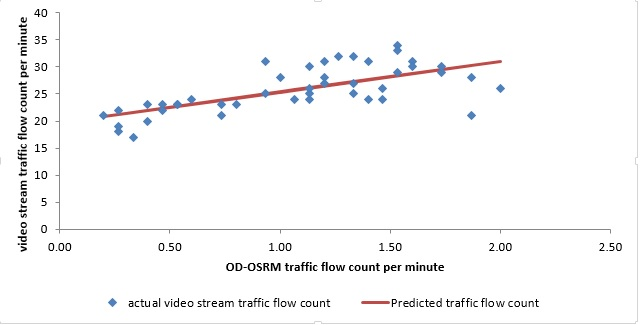
\includegraphics[width=\linewidth]{traffic_flow_count_KN_line_plot.jpg} 
		\caption{\scriptsize{OD-OSRM and video stream traffic flow Count linear plot - Kappara North}} \label{fig:traffic_flow_count_KN_lineplot}
	\end{subfigure}
	
	\vspace{1cm}
	\begin{subfigure}{0.8\textwidth}
		\centering
		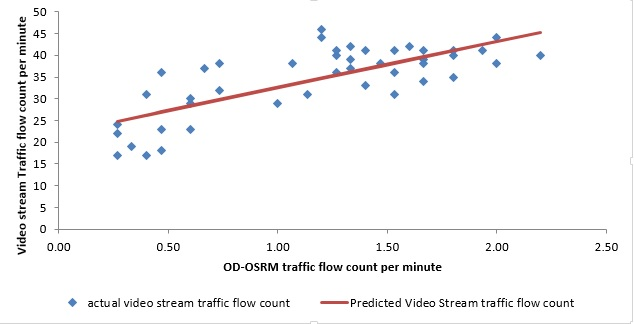
\includegraphics[width=\linewidth]{traffic_flow_count_KS_line_plot.jpg} 
		\caption{\scriptsize{OD-OSRM and video stream traffic flow Count linear plot - Kappara South}}
		\label{fig:traffic_flow_count_KS_lineplot}
	\end{subfigure}
        \caption[Linear plot for Kappara northbound and southbound traffic flow regression model]{OD-OSRM and video stream traffic flow Count linear plot for Kappara traffic flow points.}
        \label{fig:kappara_traffic_flow_count_plot}
\end{figure}

\begin{figure}[!] 
	\centering
	\begin{subfigure}{0.8\textwidth}
		\centering
		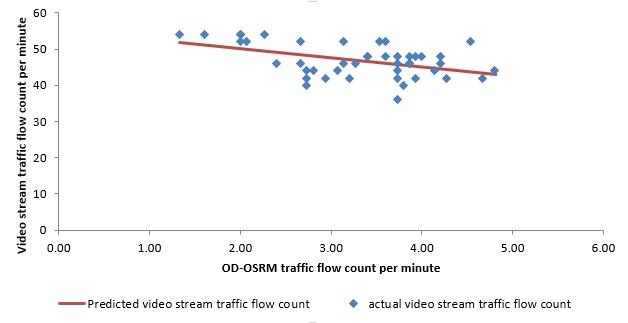
\includegraphics[width=\linewidth]{traffic_flow_count_MN_line_plot.jpg} 
		\caption{\scriptsize{OD-OSRM and video stream traffic flow Count linear plot - Marsa Northbound}} \label{fig:traffic_flow_count_MN_lineplot}
	\end{subfigure}
	
	\vspace{1cm}
	\begin{subfigure}{0.8\textwidth}
		\centering
		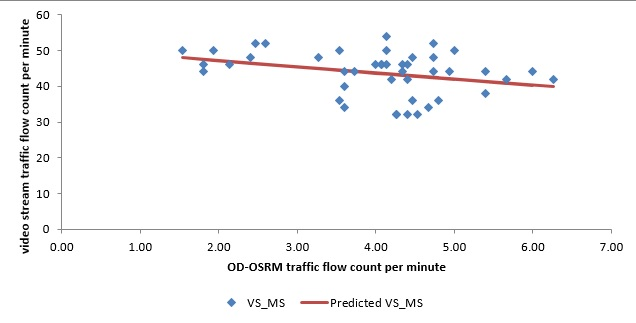
\includegraphics[width=\linewidth]{traffic_flow_count_MS_line_plot.jpg} 
		\caption{\scriptsize{OD-OSRM and video stream traffic flow Count linear plot - Marsa Southbound}}
		\label{fig:traffic_flow_count_MS_lineplot}
	\end{subfigure}	
	\caption[Linear plot for Marsa northbound and southbound traffic flow regression model]{OD-OSRM and video stream traffic flow Count linear plot for Marsa Northbound and Southbound traffic flow points.}
	\label{fig:marsa_traffic_flow_count_plots}
\end{figure}

%-----------------------------------------------------------------------------------------

A simple linear regression model was fitted for each location to analyse the type of relationship between the OD-OSRM traffic flow counts and actual traffic flow count data used from \cite{Pace2017}. There is no implied cause and impact relationship. We attempted to determine whether a true actual traffic flow count can be determined with a linear regression model from OD-OSRM traffic flow data. The resulting models were evaluated to determine how the independent variables which are location OD-OSRM traffic flow counts explain the variance of actual traffic flow. The null hypothesis here was that there is no significant functional mapping of actual traffic counts by OD-OSRM traffic counts for any specific road section.


\begin{table}[!]	
	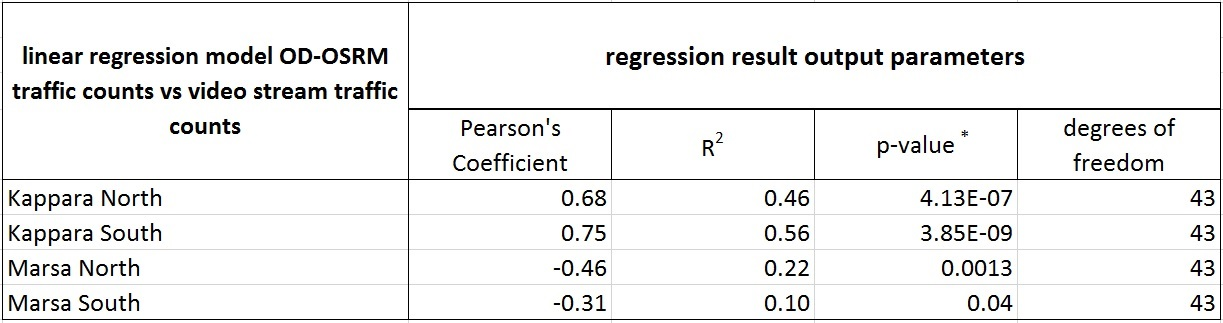
\includegraphics[scale=0.4]{traffic_flow_counts_correlation_results.jpg}
	\centering
	\caption[Correlation statistics for traffic flow linear regression models]{Correlation statistics for linear regression models. OD-OSRM traffic flow count is the predictor variable and video stream traffic count is the dependent variable. $^*$Results are all significant with $p < 0.05$.}
	\label{table:traffic_flow_correlation_results}
\end{table}

Results include Pearson's correlation coefficient, $R^2$ which indicates the explained variance and p-value which shows that all results are statistically significant. Degrees of freedom value was 43 for each directional flow under study since there was one independent variable and 44 sample data points were available for each traffic flow point under examination. These results are shown in Table \ref{table:traffic_flow_correlation_results}. 

From the results' table one can conclude that there is a strong correlation between OD-OSRM and actual traffic flow counts for both Kappara carriage ways. The strong correlation is well illustrated with line plot shown in Figure \ref{fig:kappara_traffic_flow_count_plot}. Line charts presented in Figure \ref{fig:kappara_north_traffic_flow_line_chart} and Figure \ref{fig:kappara_south_traffic_flow_line_chart} that illustrate traffic count for both Kappara carriageways show that traffic fluctuation patterns are very similar. On the contrary there is a weak negative correlation for Marsa traffic flow points (see Table \ref{table:traffic_flow_correlation_results} and line plots in Figure \ref{fig:marsa_traffic_flow_count_plots}). In fact, when we analysed traffic flow charts in Figure \ref{fig:marsa_north_traffic_flow_line_chart} and Figure \ref{fig:marsa_south_traffic_flow_line_chart},  we found that while actual traffic flow count starts high at 6.00 a.m. and gradually slows down up to 9.00 a.m. in OD-OSRM traffic flow charts shows that traffic increases constantly and peaks at 7.30 a.m. and then it starts to decrease for the subsequent later averaged samples. Traffic flow in Marsa traffic points does not necessarily mean that traffic flow is slowing down because there is less traffic load. It could be the case that traffic is slowing down because of an increase in traffic congestion \cite{Pace2017}.

Our explanation as to why there is strong correlation with Kappara traffic flows but a weak negative one with Marsa located traffic flows can be based on the fact that traffic tends to be slower in Marsa traffic flow points when compared with the Kappara traffic flow points. OD-OSRM measurements are based on trips that have been detected but if actual vehicular traffic slows down due to congestion the OD-OSRM traffic flow count does not reflect actual traffic counts. Therefore, two conclusions are derived from this. A first conclusion is that reliable regression models can be trained on actual traffic data for traffic flow road sections which do not experience heavy traffic slow down.  Secondly the regression model mapped traffic flow counts gives a reliable account of what flow capacity is expected to be serviced at any given point in time from a given road section in order that traffic flows smoothly. 

\section{Traffic flow count prediction for a selection of locations evaluation}

In Section \ref{section:traffic_flow_modelling_and_prediction}, an approach on how to predict traffic flow count for specific road sections was presented. The model proposed is an MLPC that as a function takes the traffic flow count from each recorded location as input and predicts an approximated traffic flow count for a specific location/road section for a date time in the immediate future. The traffic flow counts are binned using specific labels through a logarithmic function. 

Traffic flow count is represented with 4 bins which are equivalent to the model's classes. These classes range from class one to class four with class one being the lowest indicator of traffic flow count and class four being the highest. The MLPC model was devised by dedicating 60\% of the data for training and 40\% of the data for testing. Since Neural networks require a lot of data to train properly no data was dedicated for validating the models when searching the optimal hyper  parameters such as neural network topology layout and PCA's first k components. A trial and error approach was used to check how the model would perform when changing such hyperparameters. Testing was done only for the application phase to evaluate how the model would perform with real-world data. 

\begin{table}[t!]	
	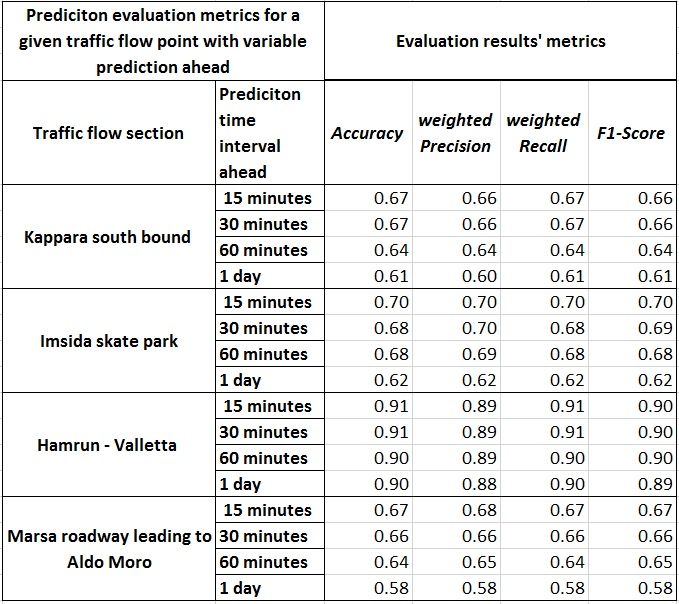
\includegraphics[scale=0.75]{classification_metrics_result.jpg}
	\centering
	\caption[Classification evaluation metrics for traffic flow prediction]{Classification evaluation metrics for 4 traffic flow road sections with 4 label classification and PCA set to extract 324 first components. Testing was done with 4 sizes of prediction time window ahead for each prediction location.}
	\label{table:classification_mertrics}
\end{table}

Collected performance metrics included accuracy and weighted precision, recall and F1-score. Accuracy gives a very basic picture of how the model is performing, however it does not provide clear information how the model is performing across all traffic flow count classes. The locations chosen from the available dataset possess the property of unbalanced classes. For example if a given location has 95\% of classes of type one a model which always predicts class one will be 95\% accurate on testing. Weighted precision and weighted recall further describe the performance of the model. When having a high precision and a low recall the model is more appropriate for exactness in classification (false positives are kept at a minimum at the cost of a high number of false negatives). A high recall and low precision model is better in identifying  a higher percentage of classes correctly but can output a relatively high number of false positives in the process.   

\begin{figure}[h]	
	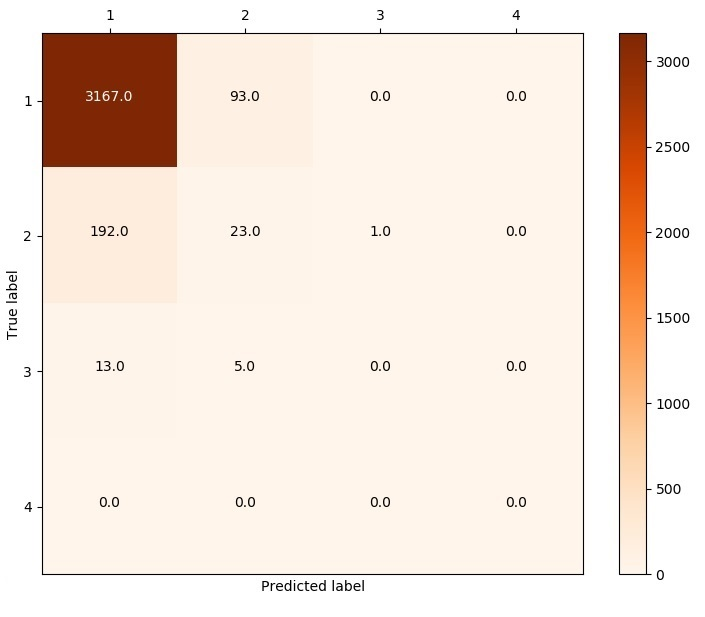
\includegraphics[scale=0.7]{confusion_matrix_hamrun_valletta_342_4bin_15min.jpg}
	\centering
	\caption[Confusion matrix Hamrun to Valletta traffic flow prediction]{Confusion matrix for Hamrun to Valleta road traffic flow count for 15 minutes ahead prediction interval.}
	\label{fig:confusion_matrix_hamrun_valletta_15min}
\end{figure}

\begin{figure}[h]	
	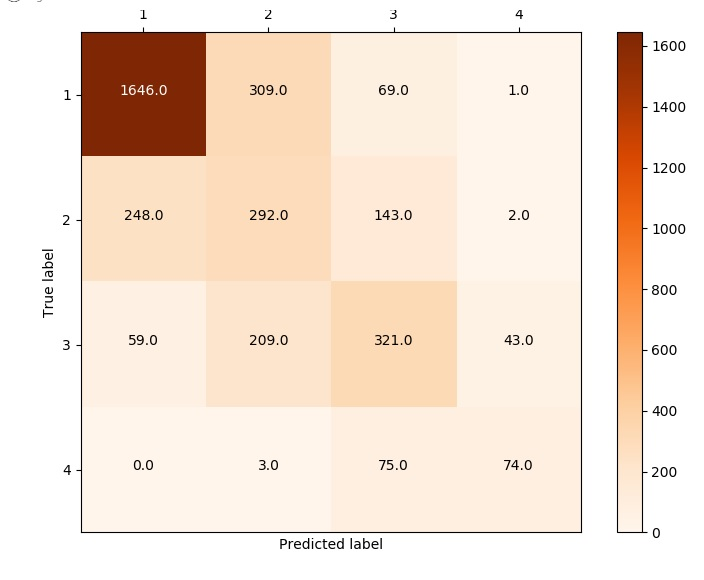
\includegraphics[scale=0.7]{confusion_matrix_marsa_aldo_moro_342_4bin_15min.jpg}
	\centering
	\caption[Confusion matrix Marsa to Aldo Moro traffic flow prediciton]{Confusion matrix for Marsa to Aldo Moro road traffic flow count for 15 minutes ahead prediction interval.}
	\label{fig:confusion_matrix_marsa_aldo_moro_15min}
\end{figure}

In machine learning sometimes high recall is more important than high precision or the other way round and in most of the times there is a trade-off. The more tuning is made to any one of the metrics to improve it, the riskier it is to get a lower performance in another metric.  The ideal is to have both high recall and high precision. In the case of this study recall for high level of traffic classes is very important since knowledge of high traffic count is important and noise would be acceptable. Weighted F1-score was used to portray a balanced measure between recall and precision.

Table \ref{table:classification_mertrics} shows the evaluation results described in terms of the metrics just discussed. It can be seen that models trained to predict for smaller time ahead intervals generally perform better than models that are trained with a lengthier prediction time interval for the same location.  Models all have proven to have highest recall and precision for class one traffic flow counts. It appears from table that the best overall classification metric scores were attained for Hamrun-Valletta roadway. However on examination of the confusion matrix (shown in Figure \ref{fig:confusion_matrix_hamrun_valletta_15min}) for classification results per label we noted that the model performed very badly for high traffic flow count classes. There were no results for class four and for classes two and three the precision and recall metrics are very low. In fact, when computing the F1-score for class two and class three, both result to be low at 0.14 and 0.0 respectively. This was found to happen as well in literature. In \cite{lv2015traffic} it is stated how trained ANN model does not perform well when traffic counts are low. Relative error in evaluation is much bigger when traffic flow is small. Results are only being quoted by Lv et al when traffic flow is 450 vehicles or more for a 15 minute time window.

In contrast predictive overall results for Marsa road that leads to Aldo Moro are less promising than those for Hamrun-Valletta arterial road. Still, the predictive efficacy results are very good, especially when examined in the perspective of the confusion matrix shown in fig. \ref{fig:confusion_matrix_marsa_aldo_moro_15min}. Class four cases, which are classified as class one or class two cases are very few and, even if almost half of class four test values were predicted as class three, in practice, this would still make the model useful and offer guidance to describe the level of high traffic flow counts.


\section{Conclusion}

This chapter demonstrated how the proposed techniques were evaluated. We have seen how there is a very strong correlation of 0.94 between global average trip count per hour  distribution which was determined with our method and the one reported in NHTS. This may indicate that our model which is derived from mobile usage data is highly relevant for the real world with assured performance. Our model has an edge on surveys similar to NHTS because the illustrated trip count per hour statistics have seasonality and the model can be updated frequently.  

Global trip delay was evaluated against data collected from Google's DMAPI. 4 routes were used for testing and correlation statistics were compiled. A very strong correlation of 0.78 exists between the average trip delay computed with our method and DMAPI average trip delay. 

When building models to express a linear regression between our method and manual data collected from video streams by Nigel Pace we saw that there was a strong correlation between models for Kappara South and Kappara North roadways but a week negative correlation with Marsa Hamrun bypass North and South roadways. We concluded that a linear regression model can be used to accurately upscale traffic flow count data from our method for a given road section, only if the road section does not experience traffic congestion frequently.

We evaluated the prediction with a MLPC by dedicating 40\% of the data for testing. Performance metrics were different for the 4 locations for which prediction testing was done. The highest F1-scores were achieved for Hamrun to Valletta route traffic flow prediction but on further scrutinizing the confusion matrix a heavy imbalance of classes towards class 1 was the reason why good prediction results were observed. The Hamrun to Valletta predictive model in fact did not perform well for classes that represent higher traffic flow counts such as Class 2 and Class 3. For other locations promising results were observed with a generally strong F1-score for all the classes. The models performed better when predicting from a shorter interval before. 



\chapter{Conclusion} \label{chapter:conclusion}

In this dissertation we described a systematic approach from which a data processing pipeline was devised to extract vehicular traffic patterns from mobile usage data. A cascading data processing pipeline methodology was used which consisted in building models for each pipeline phase that processed input data and fed next phases down the chain. The ensuing ensemble of techniques can be applied to deduce traffic analytics from time series mobile usage data. 

The aforementioned pipeline models include users' activity hubs clustering, OD matrix based trip generation, trip delay information and traffic flow measurement and prediction. Density based clustering was used to create an OD matrix containing data on visits done to the two top locations, defined as the two places where users made most use of mobile data. Trips were generated between every recorded departure from origin and arrival to destination and the resulting trip duration. OSRM was used to retrieve routes for these trips and get the actual estimated trip duration without traffic. The difference between the OSRM trip duration and the actual trip duration recorded from OD trip generation was considered to be the trip delay statistical information. OSRM was used as well to collect time series data that indicated where the traffic flow is being distributed on the road infrastructure in order to build aggregate statistical models. The traffic flow counts' dataset then was used to train an MLPC to build a model that predicts traffic flow count at varied time intervals ahead.

Clustering was the only part of the methodology that could not be evaluated directly. Ground truth was not available to test how  accurately the resultant main locations for each user were matching the actual ones. Its evaluation relied on traffic flow count evaluation which is highly dependent on the OD-OSRM generated trips which are defined by the users' main two clusters.

Since the mobile users population does not match the number of commuters that use their own vehicle for transportation it was expected that trip distribution statistics would give lower values than those reflected by actual values. A scaling up method was needed to extrapolate real world trip distribution statistics. A very strong correlation of 0.94 was found between average NHTS 2010 trip distribution data and trip distribution generated by the OD-OSRM method devised in our research. A linear regression model was built to map OD-OSRM figures to scaled up numbers. One should underline the fact that a lot of human resources are needed to collect survey data and that surveys become eventually outdated. The method proposed in this research can use readily available data, can have its model dynamically updated and can be configured with a 5 minute temporal resolution. Survey responses may not contain exact departure and arrival times since people possibly tend to round these when replying. Therefore, as a conclusion our method is more practical than surveys to get information on user trips. However, it needs to be calibrated and scaled up by modelling on actual surveys through regression. This, however, does not need to be done frequently. 

Correlation statistics were carried out for trip hourly average delay for four different routes. A promising overall correlation of 0.72 was found between trip delay data originating from OD-OSRM and Google's DMAPI. However one must note that DMAPI data was collected for a week in the month of June 2018 and OD-OSRM data was collected in October 2016. Our approach seems to work better to give predictive models for the distant future because Google's model for the distant future gives identical results to those given for the immediate future. Our method can be easily modelled with seasonality to forecast distant traffic delay if a year of data is available.

Traffic flow distribution linear regression models were built to map OD-OSRM traffic flow distribution to actual ones. The linear relationship with data collected manually for four locations was analysed. It was concluded that the linear relationship is statistically significant and tends to have high correlation if the road traffic flow capacity is not exceeded. Otherwise for locations that tend to have high traffic congestion, correlation is both low and negative during traffic congestion time. Therefore, it was concluded that negative correlations in traffic flow distribution linear models indicate that locations are experiencing slowing down of traffic due to congestion.

Machine learning techniques were employed to predict traffic flow counts at a given time for a given location from previous traffic flow counts at an earlier time for all location data points. An MLPC was trained for four locations and prediction intervals ranged from 15 minutes to 1 day. Satisfactory results were attained and from these results it is concluded that users or information support systems can make well informed decisions on predicted traffic flow data for selected locations.

The main strength of this dissertation was to give an accurate measure and an effective prediction of traffic flow demand (not traffic congestion) on the road infrastructure. The insight gained could help transport agencies' administrators to tackle infrastructure problems before they eventually happen. Improvement is mainly needed on dynamic traffic assignment algorithms.

\section{Major contributions of this dissertation} \label{section:major_contributions}

This research posed questions on whether it is feasible to get vehicular traffic descriptive and predictive analytics from mobile usage data. We showed how it is possible to retrieve top activity locations for users. It is possible also to achieve accurate results in getting global trip counts and trip delays. From mobile data usage as well, we have shown that it is possible to collect trip data for all users. The trip data was then used to actually map traffic flow demand on the road grid. However, it was found that traffic flow mapping gave accurate results for low traffic congestion roads, whereas for high traffic congestion roads our model did not give accurate results. Finally, a MLPC was found really efficient to predict traffic flow for a set of locations. The confidence level given by the prediction results is high and if traffic flow input used to train the predictive model is accurate the method we devised could be used in the real world to forecast traffic in real-time. We did not experiment with processing of real-time streams but the model we devised can be easily adapted for real-time processing since it uses window analytics which are widely used for stream processing.


\section{Discussion} \label{discussion}

In this research machine learning was used to train an MLPC with all locations' traffic flow count as data features. All the traffic flow count would be mapped by a built model to a level of traffic representing the future traffic flow count for a specific location. A similar predictive model can be built to predict estimated trip delay for every given route for any given required time. A comprehensive used routes database that exists in Malta for all users based on the OD matrix has to be compiled. Then statistical information on trip delays per 5 minutes for same routes are aggregated. One should investigate the possibility of using routes' trip delays as training input features to a machine learning model. The final predicted classification would be a trip delay class for certain give routes. The model basically would be a function that maps trip delays for a set of routes to a classification of trip delay for a given route.

In order not to increase the evaluation combinations only two main clusters' location were retrieved per user. These two clusters were considered as being the home and work locations. However the main relevant assumption was that most trips were made between these two main clusters. This is not representative for all trips made and would incur phantom trip delays that could only be explained by stops at locations frequently visited by users that are not one of the main activity clusters. A fact that heavily impacts daily traffic in Malta are extra trips whose destinations are concentrated around schools. School run trips can be detected by extracting the third most common location that is located within a school geofencing boundary and by time boxing with school starting and finishing hours. A lot of trips have been discarded with the used methodology because they had excessive delays. Many of these trips can be retained to better explain the traffic dynamics if trips are further divided with the insertion of a third location.

Other datasources such as social media and ANPR video streams could be used to further dynamically assign traffic to the road network. From social network feeds one can extract for example accidents location and time. This data could be used to analyse the accident impact on traffic flow and can be used as an input feature for machine learning models. Also correlation between weather and traffic flow can be done by using available weather APIs.

This dissertation's methodology made extensive use of Open source maps (OSM) and Open Source Routing Machine (OSRM). An interesting project would be to edit the OSM maps under observation (opening of a new road) with map editing software and check the impact on the traffic flow of routes which are adjacent or near to the modification done in the map. OSRM generates route information based on the OSM data and when the OSM data file is modified the change is reflected in the routing information. This would be very useful to simulate and analyse the impact on traffic flow before the actual alteration is made in the road infrastructure. 

\chapter{Future Works} \label{chapter:future_work}

This dissertation created a lot of experimental data while developing and evaluating techniques which can be the background for future projects. Features suggested in this chapter were not investigated due to time constraints. Future works are categorized into two namely, future improvements and future research.


\section{Future improvements} \label{section:future_improvements}


The challenge in such projects is to find ground truth to properly evaluate findings and achieved results. One way to achieve this is to develop or use off the shelf software that collects GPS points and collaborate with a group of people to gather the data. The resulting sample of data would be ideal to carry out correlations with experimental outcomes.

DBSCAN was used to find density based clusters to extract the most common origin and destination locations for users. As discussed in Section \ref{section:methodology:clustering}, $\epsilon$ was set to 500m. OPTICS is an algorithm which is similar to DBSCAN but it does not require $\epsilon$ parameter as an input and is more efficient to find meaningful clusters for data with varying density \cite{Ankerst1999}. Clusters generated on data used in this research and that had a weak density might have not been captured with a radius of 500m. DBSCAN was furthermore computationally expensive and consumed a lot of time in the experimentation phase. An optimization for the performance of the processing of the whole pipeline would be running DBSCAN on data in parallel in a distributed manner. An implementation based on the Spark platform is proposed in \cite{huang2017research}.

One limitation in this dissertation was to assume that users always take the fastest route and do not detour for whatever reason along the trip. Traffic assignment therefore is static and does not adapt to the traffic events on the road infrastructure. This does not give optimal results when gathering real-time and historical analytical statistics on routes, trips and distributed traffic load on the road infrastructure. Other methods must be combined with the proposed solution to rectify route selection and give a more realistic picture of traffic flow based on actual user route taking. 

One way how to improve the correct route selection rate is by further polling mobile usage data during a user trip and snap the user to the nearest road route with snap to road software such as Roads API from Google\footnote{https://developers.google.com/maps/documentation/roads/snap (accessed January 8, 2018)}. This type of software takes a set of coordinates as input and returns a similar set of data that most likely define the route outlined by the set of data. Route selection would not be necessarily computed for each user every time a user trip is detected. A statistical model can be built to learn what are the most likely routes taken by each user on a given date and time context. This model can then be used in the application phase to analyse traffic loads which are related to the predicted routes.

An averaging moving filter could be used to remove noise from the traffic flow count and improve results by applying a smoothing function. When getting a sliding average more data points can be used for prediction. In our approach to reduce computational costs, an average with binning size of 5 minute each was calculated. This reduced however, a 60 data point resolution to 12 data points in an hour. When building a machine learning model that predicts traffic flow counts, a fixed interval was used to get the future classification label (refer to section \ref{section:traffic_flow_modelling_and_prediction}). This fixed interval had to be a multiple of the 5 minute window and there was no flexibility for more granular tuning. Having less data points for the reasons just mentioned provided less data for training to the MLPC.


Evaluation for average trip delay computation (see section \ref{section:trip_average_delay_evaluation}) was done by comparing results based on a June dataset with data retrieved through DMAPI and an October mobile data usage dataset. This evaluation although it gave promising results should be repeated with seasonality of datasets removed from the equation to compare like with like. Malta traffic in October is very different from Malta traffic in June. 






\bibliomatter
\bibliographystyle{ieeetr}
\bibliography{references}


 
\end{document}
